%10MB

\documentclass[10pt,finnish,a5paper]{scrartcl}

\usepackage[left=1.5cm,right=1.5cm,top=1.5cm,bottom=2cm]{geometry}
\usepackage{fontspec}
\usepackage{babel}
\usepackage{microtype}
\usepackage{multicol}
\usepackage{xcolor}
\usepackage{enumitem}
\usepackage{ragged2e}
\usepackage{graphicx}
\usepackage{wallpaper}
\usepackage{lipsum}
\usepackage[labelformat=empty]{caption}
\usepackage[export]{adjustbox}
\usepackage{calc}
\usepackage{pstricks}
\usepackage{contour}
\usepackage{multirow}
\contourlength{2pt}

\usepackage{draftwatermark}
\SetWatermarkText{\textbf{LUONNOS}}
\SetWatermarkScale{1}

\newenvironment{Figure}
  {\par\medskip\noindent\minipage{\linewidth}}
  {\endminipage\par\medskip}

\definecolor{link}{HTML}{f7941e}

\RedeclareSectionCommands[tocraggedentrytext]{section}

\setlength{\RaggedRightParindent}{\parindent}
\RaggedRight
\setmainfont[Ligatures=TeX]{Ubuntu}
\newfontfamily\monofont{Ubuntu Mono}
\definecolor{kuru}{HTML}{f7941e}
\setcounter{secnumdepth}{0}
\setcounter{tocdepth}{2}
\addto\captionsfinnish{\renewcommand{\contentsname}{Tässä numerossa}}
\addtokomafont{sectionentry}{\normalfont}
\addtokomafont{disposition}{\rmfamily\color{kuru}}
\addtokomafont{caption}{\footnotesize}
\setkomafont{subsection}{\normalfont\itshape}
\setenumerate{leftmargin=*}
\setitemize{leftmargin=*}
\frenchspacing
\def\UrlBreaks{\do\/\do-}

\usepackage[automark, autooneside=false]{scrlayer-scrpage}
\pagestyle{scrheadings}
\setkomafont{pageheadfoot}{}% not special font for page head and foot
% \clearpairofpagestyles
% \ihead{\leftmark}
% \ohead{\Ifstr{\leftmark}{\rightbotmark}{}{\rightbotmark}}
% \ohead{\Ifstr{\rightbotmark}{\leftmark}{}{\leftmark}}
\ihead{}
\chead{}
\ohead{\color{kuru}\rightmark}
% \ihead{\headmark}
% \markright{
% }
\cfoot{\pagemark}

% Packages needed:
\usepackage{tikz}
\usepackage[most]{tcolorbox}
\newtcolorbox{kuruboxtitle}[1][]{%
    enhanced,
    before skip=0mm,after skip=0mm, 
    width=1\textwidth, boxrule=0mm,
    colback=kuru, colframe=kuru, % Colors
    sharp corners,
    underlay={%
	    \fill[kuru] ([xshift=-10mm,yshift=2mm]frame.north west) -- ([xshift=8mm]frame.north east)
	    -- ([xshift=10mm,yshift=-2mm]frame.south east) -- ([xshift=-8mm]frame.south west)
	    -- cycle;
	    \fill[white] ([xshift=-6mm,yshift=-2mm]frame.north west) ellipse (1mm and 2mm);
	    \fill[white] ([xshift=-3mm,yshift=-2mm]frame.north west) ellipse (1mm and 2mm);
	    \fill[white] ([xshift=-4.5mm,yshift=-6mm]frame.north west) circle (1mm);
	    \fill[white] ([xshift=-4.5mm,yshift=-9mm]frame.north west) circle (1mm);
        },
    % drop fuzzy shadow, % Shadow
    title={#1},
}

\usepackage{titlesec}
\titleformat
{\section} % command
[display] % shape
{\bfseries\Large} % format
{\thechapter} % label
{0.5ex} % sep
{
	\clearpage
	\thispagestyle{plain}
	\begin{center}
		\begin{kuruboxtitle}[]
			\color{white}
} % before-code
[
		\end{kuruboxtitle}
	\end{center}
] % after-code

\usepackage[colorlinks,linkcolor=black,urlcolor=link]{hyperref}
\renewcommand{\theHsection}{\thepart.section.\thesection}
\urlstyle{same}

\begin{document}
\thispagestyle{empty}
\newgeometry{left=1cm}

% \ThisCenterWallPaper{1.10}{assets/no_auto_compression/kansikuva}

\vspace*{5.70cm}

{\noindent\color{kuru}\begin{tabular}{@{}c@{}}

\includegraphics[width=6cm]{assets/no_auto_compression/logo} \\
\\

\newtcolorbox{kuruboxfrontpage}[1][]{%
    enhanced,
    before skip=0mm,after skip=0mm, 
    width=0.6\textwidth, boxrule=0mm,
    colback=kuru, colframe=kuru, % Colors
    sharp corners,
    underlay={%
	    \fill[kuru] ([xshift=-8mm,yshift=3mm]frame.north west) -- ([yshift=1mm]frame.north east)
	    -- ([xshift=1mm,yshift=-3mm]frame.south east) -- ([xshift=-7mm,yshift=-1mm]frame.south west)
	    -- cycle;
	    \fill[white] ([xshift=-4mm,yshift=-1mm]frame.north west) ellipse (1mm and 2mm);
	    \fill[white] ([xshift=-1mm,yshift=-1mm]frame.north west) ellipse (1mm and 2mm);
	    \fill[white] ([xshift=-2.5mm,yshift=-5mm]frame.north west) circle (1mm);
	    \fill[white] ([xshift=-2.5mm,yshift=-8mm]frame.north west) circle (1mm);
        },
    % drop fuzzy shadow, % Shadow
    title={#1},
}
\begin{kuruboxfrontpage}[]
	\color{white}{\large\bfseries 1/2025 Kurkisuon Rusakot ry}
\end{kuruboxfrontpage}
% \contour{white}{\large\bfseries 1/2024 Kurkisuon Rusakot ry}
\end{tabular}\par}

\clearpage
\restoregeometry
\thispagestyle{plain}

% \ThisULCornerWallPaper{1}{assets/no_auto_compression/sisäkansikuva.jpg}

\noindent \textbf{Tassu 1/2025} \\
\noindent ISSN 0783-1536

\vfill

% \begin{multicols}{2}
\noindent\textbf{Päätoimittaja:}

Tanguy Gérôme

\href{mailto:tanguy@gerome.fi}{tanguy@gerome.fi}

\medskip

\noindent\textbf{Julkaisija:}

Kurkisuon Rusakot ry, Helsinki

\medskip

\noindent Tarkista lippukunnan ajankohtaiset yhteystiedot nettisivuilta:

\href{https://kurkisuonrusakot.wordpress.com/}{kurkisuonrusakot.wordpress.com}

\medskip

\noindent Etu- ja sisäkannen kuvat:

xxx

\noindent Takakannen kuva:

xxx

% \columnbreak
\vspace{0.64cm}

\tableofcontents
% \end{multicols}

\section{Lippukunnanjohtajan tervehdys}

\begin{multicols}{2}
\noindent Haarapääskyt, räystäspääskyt ja tervapääskyt ovat jo aikaa sitten
saapuneet, merihanhilla on jo poikasia ja kuuluipa pellon laidalta
tuttu harmaasiepon ''tsri tsri tsri''. Kevät on jo täällä ja kesä on
aivan kulman takana. Valkovuokko, rentukka ja kirsikka ovat täydessä
kukassa ja ensimmäiset satakielet virittävät lauluaan aamuhämärässä.
Aivan, kesällä järjestetään lippukunnan \textit{Satakieli}"-kesäleiri!
Leirin lisäksi kesän toimintaan lukeutuvat \textit{Variksen vavahdus}
"=vaellus ja \textit{Piisaminhäntä}"-melonta. Olethan sinäkin mukana
kesän partiotapahtumissa?

Alkuvuoteen on jälleen mahtunut monenlaista partiotekemistä kuten
laskiaisriehaa, minihaikkia, partioparaatia ja lippukuntaretkeä. Olen
haltioissani siitä, kuinka paljon erilaista toimintaa pieni
lippukuntamme on pystynyt järjestämään; kevään toimintamme on
kartuttanut käyntikertoja yli seitsemänsataa! Tämä ei ole mikään
itsestäänselvyys, vaan mielekäs toiminta vaatii aina vapaaehtoisia,
tekijöitä ja johtajia -- unohtamatta itse osallistujia, joita ilman
tekeminen menettää merkityksensä.  

Osin partiotoiminnan mahdollistaa se, että lippukuntamme on
rekisteröity yhdistys. Sillä on vuosikokouksen valitsema hallitus, joka
vastaa toimintasuunnitelman toteutumisesta, päättää kalusto- ja muista
hankinnoista, ylläpitää jäsenrekisteriä, anoo avustuksia, edustaa
lippukuntaa piirin aluetapaamisissa\ldots\ Lippukunnan hallinto on
yleistäen kuin valtion, kunnan tai jonkin yrityksen hallinto
pienoiskoossa, joten partiotoiminnan tähän välillä tylsältäkin
vaikuttavaan osaan tutustuminen tarjoaa johtajalle paljon hyödyllisiä
tietoja ja taitoja, joista on aikuisena hyötyä muuallakin. Haluaisitko
sinä tutustua lippukunnan hallituksen tehtäviin? Kysy lisää
allekirjoittaneelta!

Tässä Tassussa pääset palaamaan viime vuoden pikkujouluretkeen,
riihitystunnelmiin vuonna 2018 ja tänä keväänä sekä tarpojien
minihaikille. Seikkailijoiden sivuilla (s. \pageref{sec:seikkailijat})
on paljon hauskaa luettavaa ja tekemistä. Julkistetaanpa lehdessä myös
viime numeron kuvakilpailun voittaja. Ja jos et ole vielä aloittanut,
nyt on oikea hetki alkaa pohtia, kuinka oikea ja nurja silmukka oikein
tehtiinkään, ottaa neulepuikot esiin ja osallistua Tassun
neulesuunnittelukilpailuun -- lue lisää sivulta
\pageref{sec:neulekilpailu}!

{\smallskip\noindent\centering ***\par\smallskip}

Kevättä varjosti Kurkisuon Rusakoiden perustajajäsenen ja ensimmäisen
lippukunnanjohtajan, \mbox{Eddien} poisnukkuminen. ''Yritä jättää tämä
maailma vähän parempana kuin sen löysit,'' kehotti lordi Baden"-Powell,
partioliikkeen perustaja viimeisessä viestissään maailman
partiolaisille. Sama ilmaisu löytyy Suomen Partiolaisten
partioneuvoston hyväksymistä partion yhteiskunnallisen toiminnan
linjauksista. Nykyisenä lippukunnanjohtajana olen vahvasti sitä mieltä,
että Eddie otti kehotuksesta vaarin.

Partioterveisin ja Eddien muistoa kunnioittaen

\smallskip

\noindent\hfill Janne

\vspace*{12cm}

\columnbreak

\null\vfill

\noindent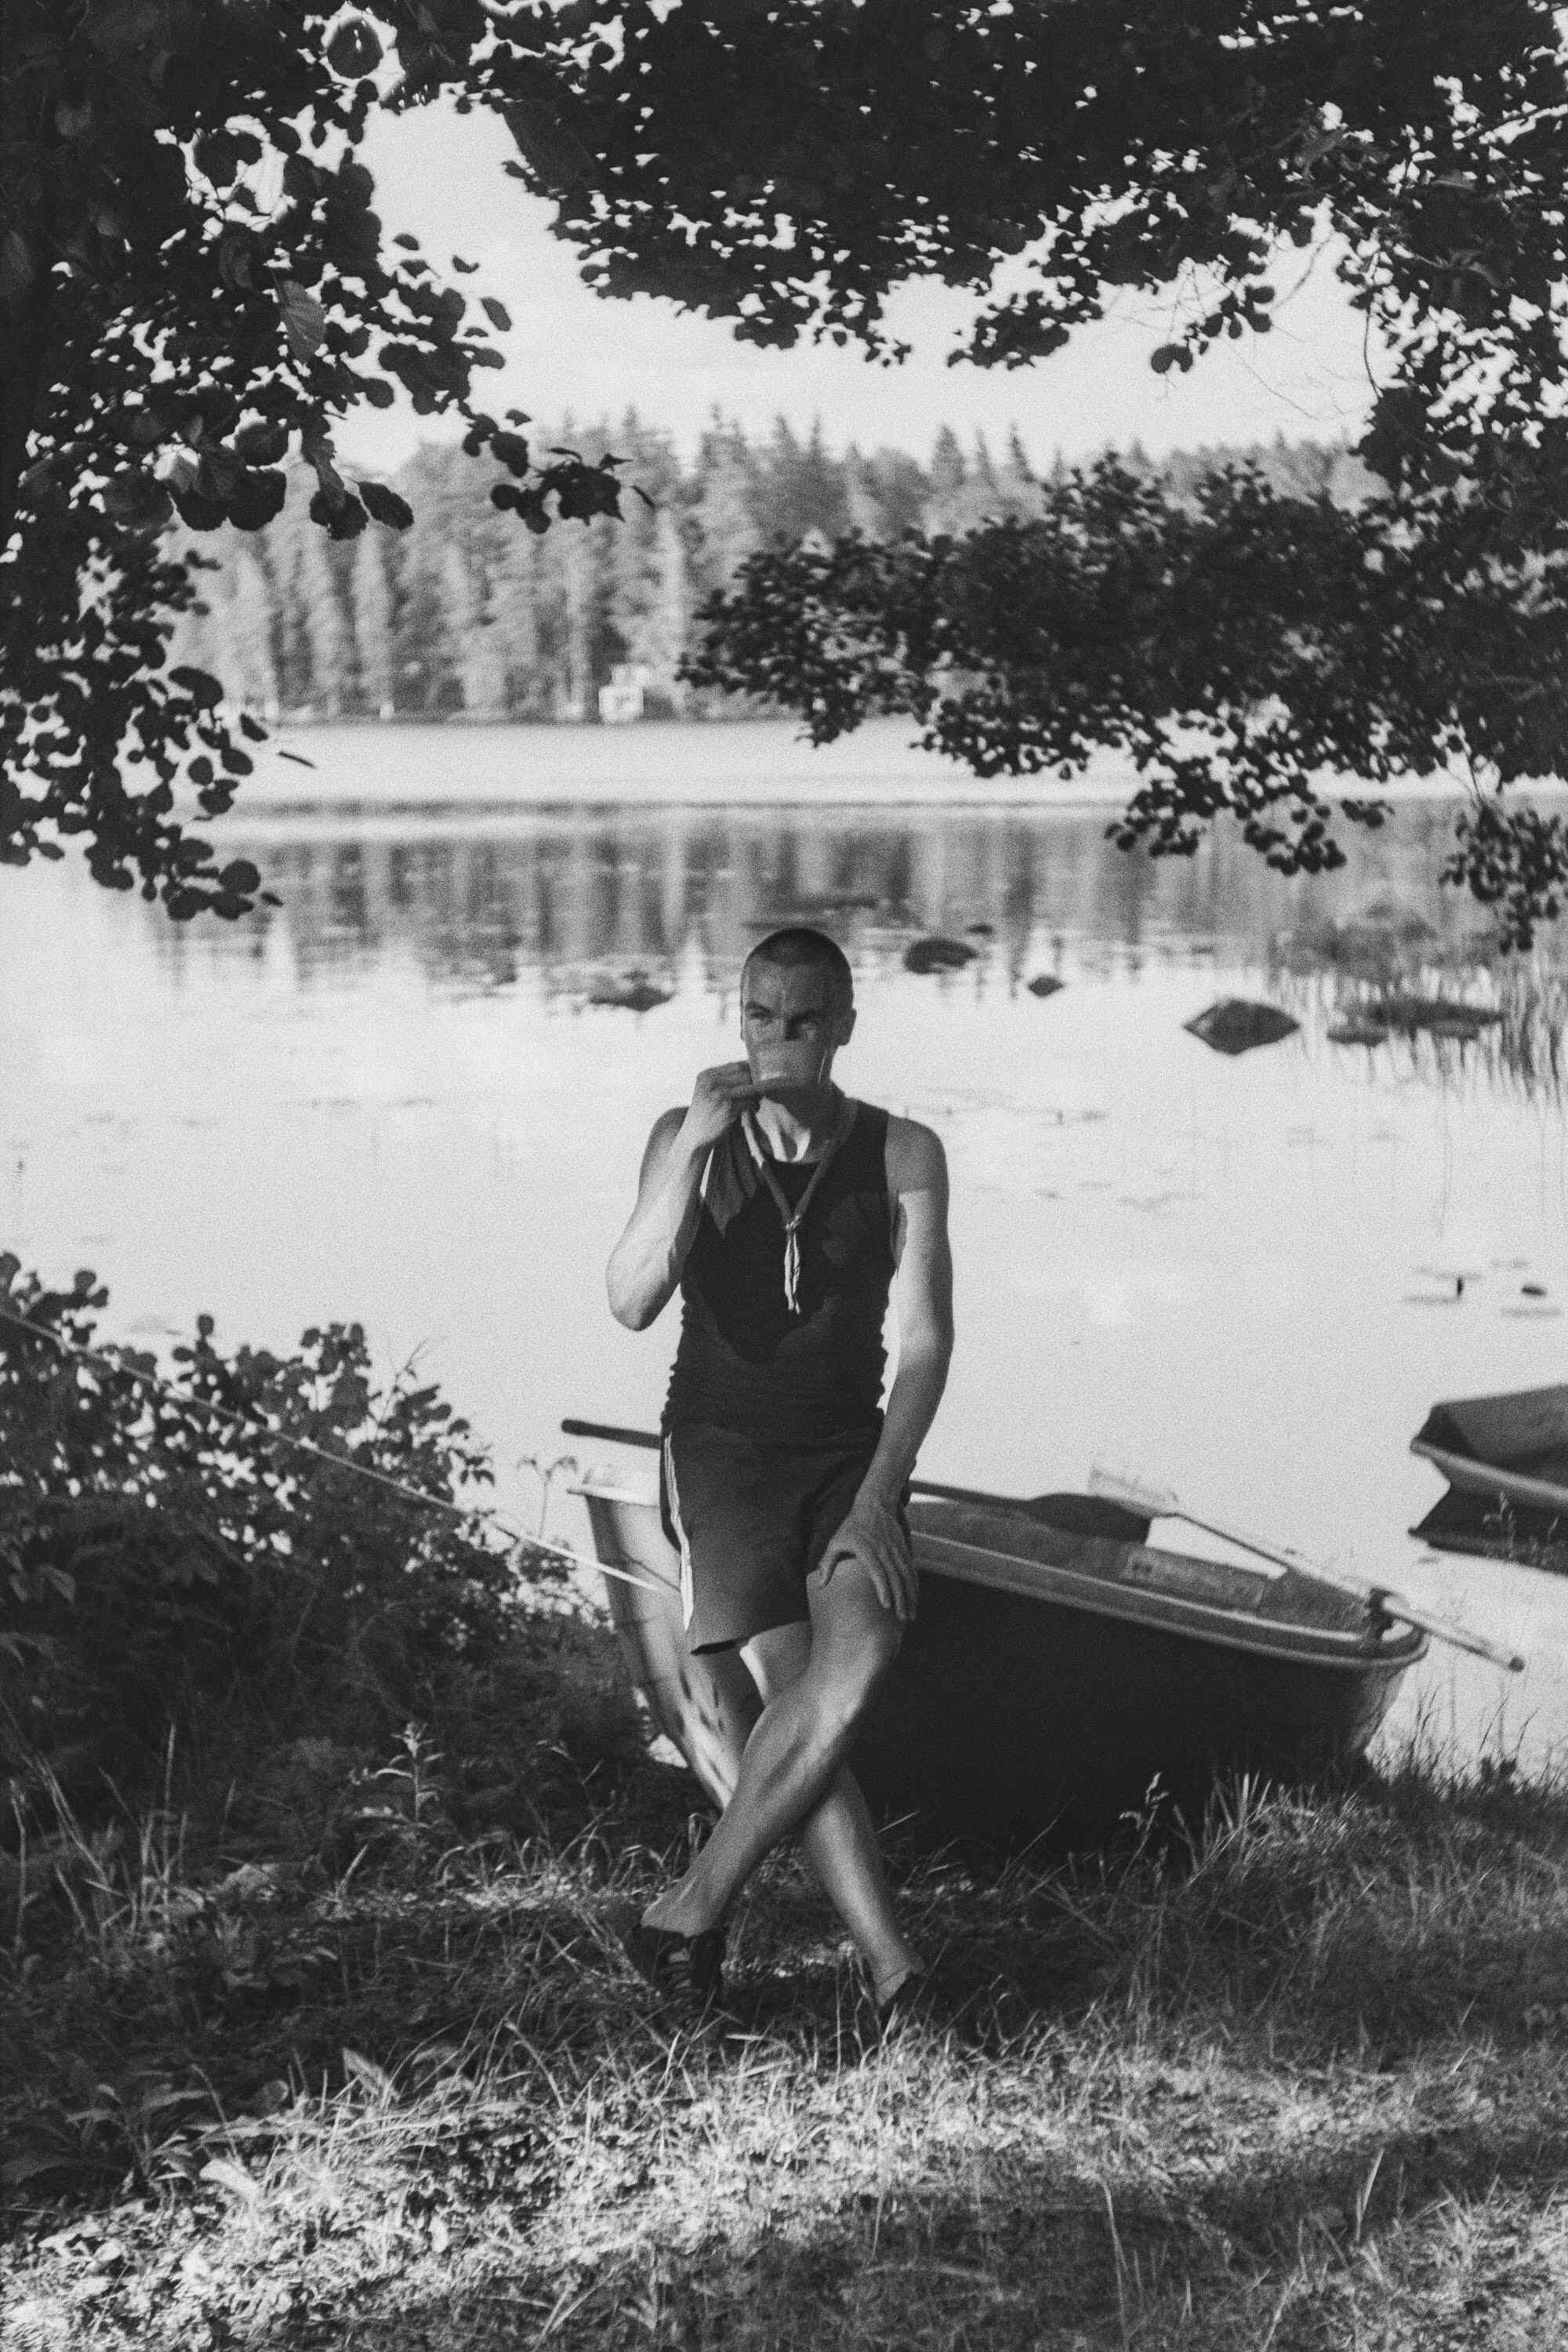
\includegraphics[width=\linewidth]{assets/lpkjohtajantervehdys} \\
{\small Lippukunnanjohtaja nauttimassa iltateestä \textit{Uikun uinti}
"=vaelluksen helteisen, kolmannen päivän päätteeksi Ruokojärven rannalla.\par}

\bigskip

\noindent\null\hfill Kuva: Tanguy
\end{multicols}



\section{Tassu ennen vanhaan}
\textit{Tassu on ilmestynyt säännöllisen epäsäännöllisesti lippukunnan perustamisvuodesta 1986
lähtien. Tällä palstalla muistellaan menneitä ja julkaistaan valittuja paloja takavuosien
lehdistä.}

% \textit{Päätoimittaja sai paketin, jossa on vuosikymmeniä Tassun painoksia ja
% yrittää digitalisoida ne lähiaikoina!}

\vspace*{0.32cm}
% \noindent Tällä kertaa mennään ajassa 20 vuotta taaksepäin, ja katsotaan mitä
% \mbox{KuRu:n} kolkat puuhasivat heidän syysretkellään vuonna 2004:

\newtcolorbox{StickyNote}[1][]{%
    enhanced,
    before skip=2mm,after skip=2mm, 
    width=\textwidth, boxrule=0.2mm, % width of the sticky note
    colback=kuru!50!white, colframe=kuru, % Colors
    attach boxed title to top right={xshift=0cm,yshift*=0mm-\tcboxedtitleheight},
    varwidth boxed title*=-3cm,
    % The titlebox:
    boxed title style={frame code={%
        \path[left color=kuru,right color=kuru,
        middle color=kuru]
        ([xshift=-0mm]frame.north west) -- ([xshift=0mm]frame.north east)
        [rounded corners=0mm]-- ([xshift=0mm,yshift=0mm]frame.north east)
        -- (frame.south east) -- (frame.south west)
        -- ([xshift=0mm,yshift=0mm]frame.north west)
        [sharp corners]-- cycle;
        },interior engine=empty,
    },
    sharp corners,rounded corners=southeast,arc is angular,arc=3mm,
    % The "folded paper" in the bottom right corner:
    underlay={%
        \path[fill=kuru!80!black] ([yshift=3mm]interior.south east)--++(-0.4,-0.1)--++(0.1,-0.2);
        \path[draw=kuru,shorten <=-0.05mm,shorten >=-0.05mm,color=kuru] ([yshift=3mm]interior.south east)--++(-0.4,-0.1)--++(0.1,-0.2);
        },
    % drop fuzzy shadow, % Shadow
    % fonttitle=\bfseries, 
    title={#1}
}

\vspace*{0.64cm}
\begin{StickyNote}[Julkaistu alunperin Tassussa x/xxxx]
	\monofont

\end{StickyNote}


% \section{Muistoja vuodelta 2023: Johtajien kansallispuistokierros Ruotsissa}
% \section{Muistoja vuodelta 2024: Uikun uinti -vaellus 26.–30.6.}

\section{Eläinten joulu Meriharjussa}

\textit{Gustaf Björkenheimin rakennuttama Villa Meriharju on vuonna 1910 
valmistunut huvila Uutelassa. Nykyään huvila on Helsingin kaupungin 
omistuksessa ja se kulkee nimellä Meriharjun luontotalo. Rusakot ovat tehneet 
pikkujouluretkiä luontotalolle jo useamman kerran, vuosina 1996--2001, 2003, 
2008, 2009, 2015, 2016 ja 2019--2023. Myös vuoden 2024 pikkujouluretki 
suuntautui Meriharjuun -- lue lisää retken tapahtumista tästä jutusta!}

\begin{figure}[!b]
\centering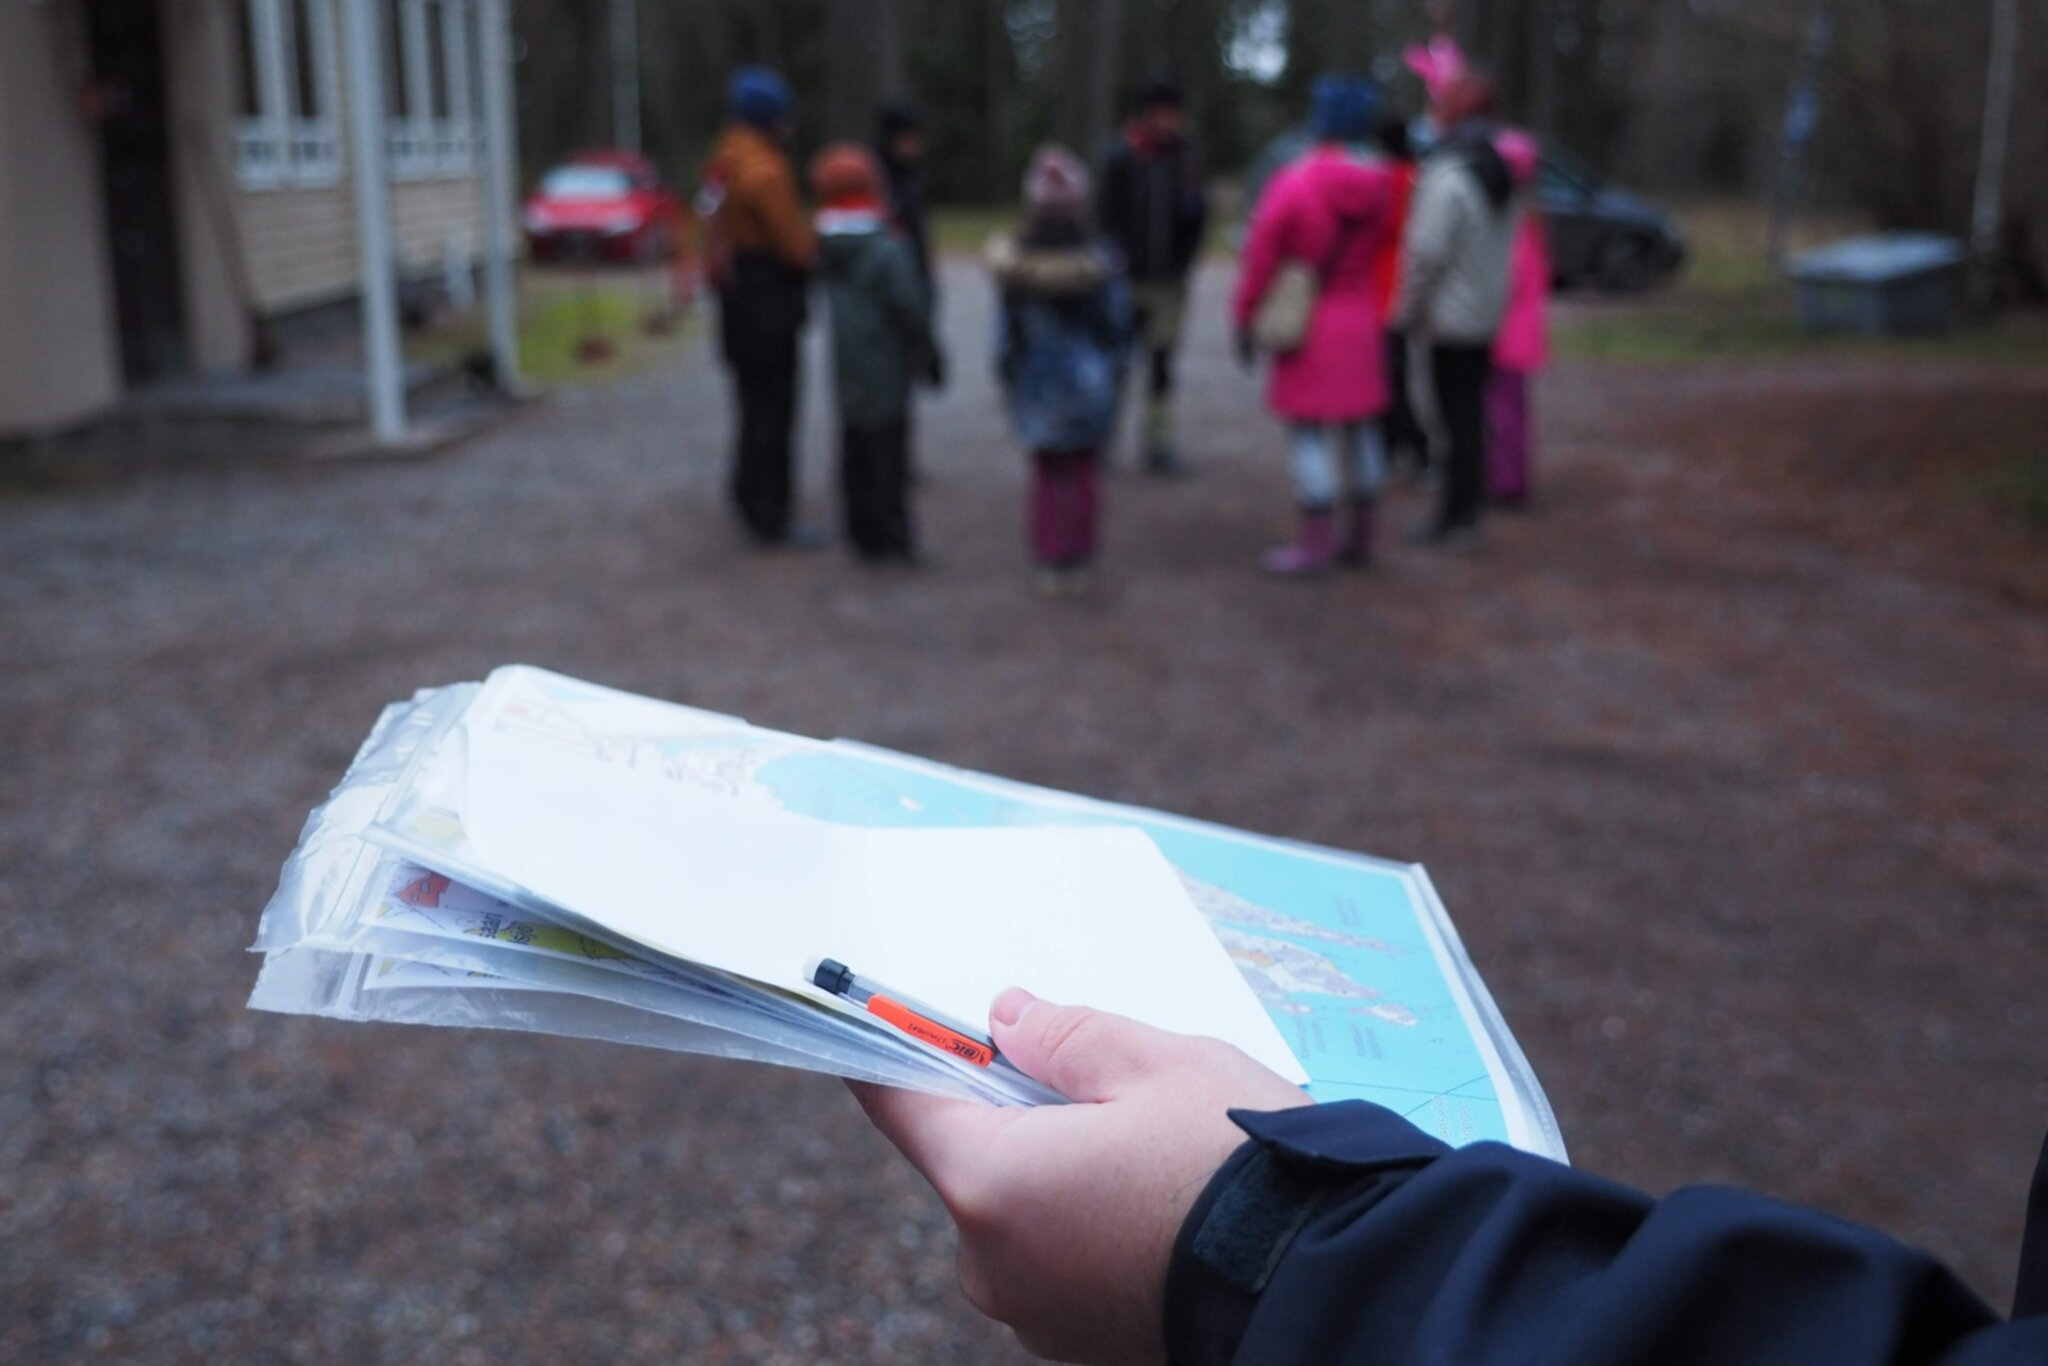
\includegraphics[width=\textwidth]{assets/meriharjuSuunnistus}
\caption{Lippukuntaretken lauantaisuunnistus käynnistyi luontotalon edustalta.}
\end{figure}

\begin{multicols}{2}
\noindent Kautta aikain rusakoiden pikkujouluretkillä on ollut erilaisia 
teemoja. Viime vuosina teemoina ovat olleet Itämeri, lentokykynsä 
menettäneet joulupukin porot, Kalevalan joulu sekä karanneet ja vilustuneet 
lehmät. Rusakoiden Meriharjun 17. pikkujouluretken teemana oli metsän 
eläinten joulu. 

\begin{figure*}[!t]
\centering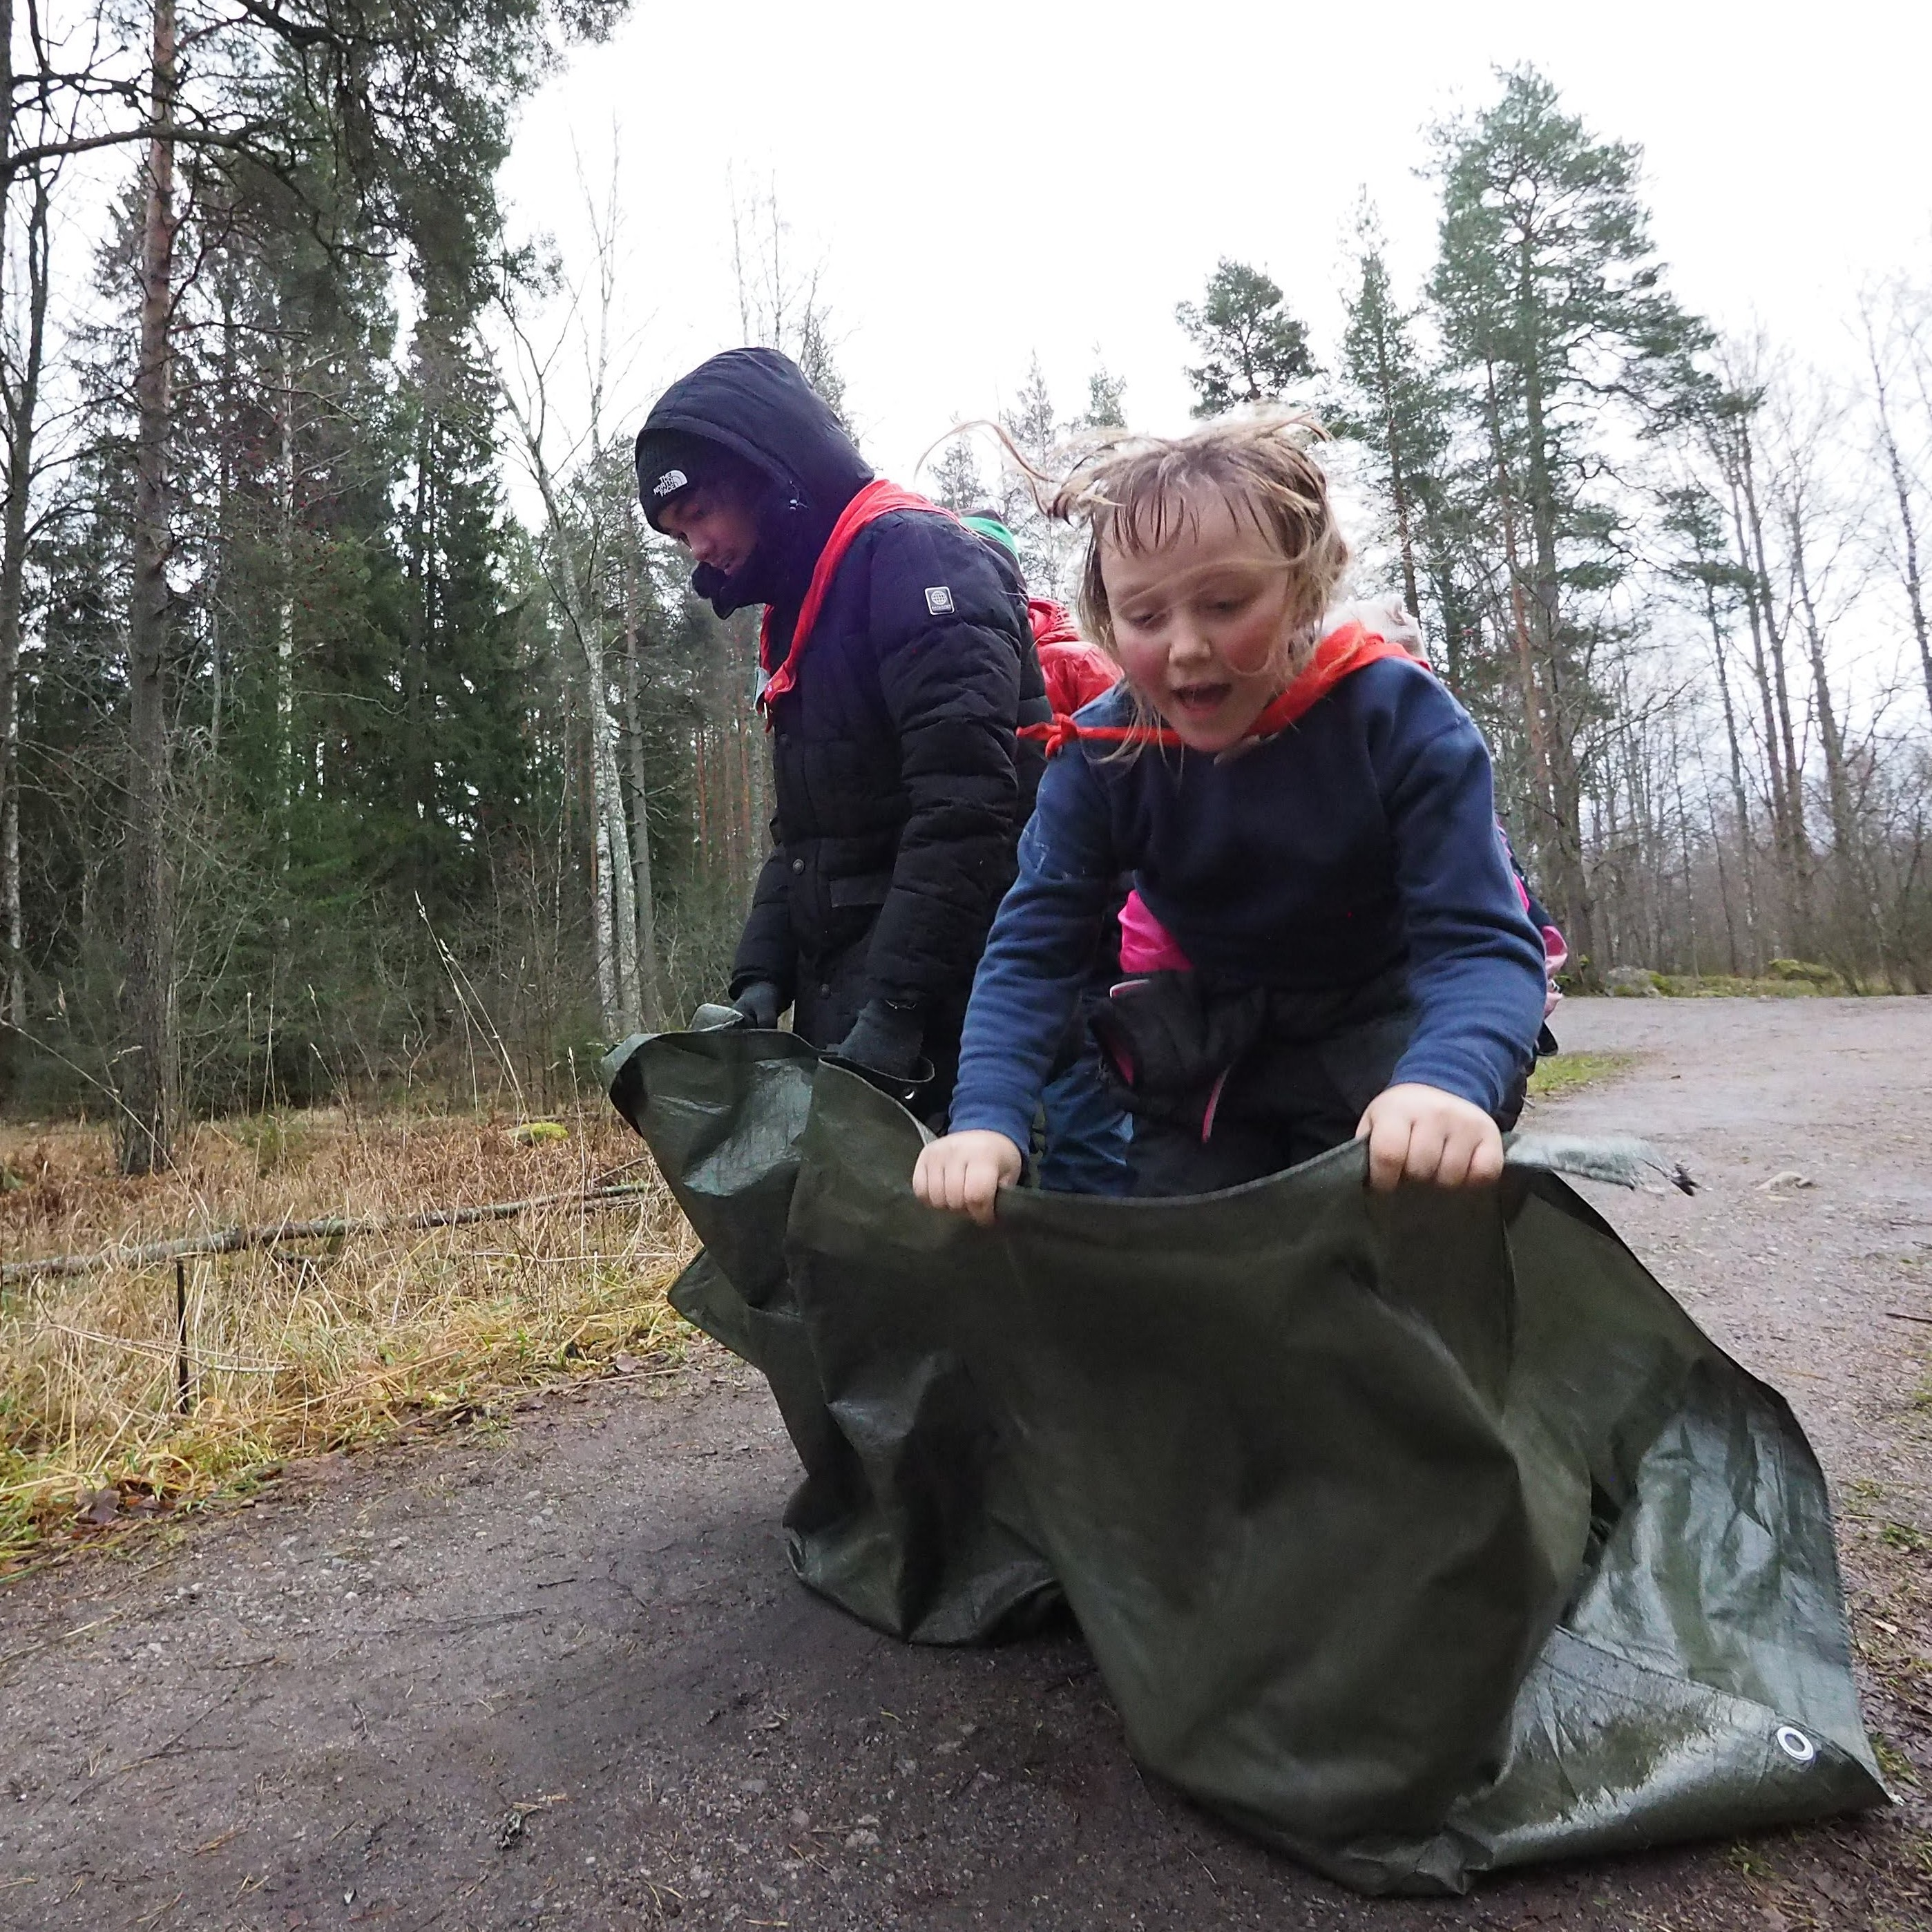
\includegraphics[width=.475\textwidth]{assets/meriharjuTaikamatto}\hfill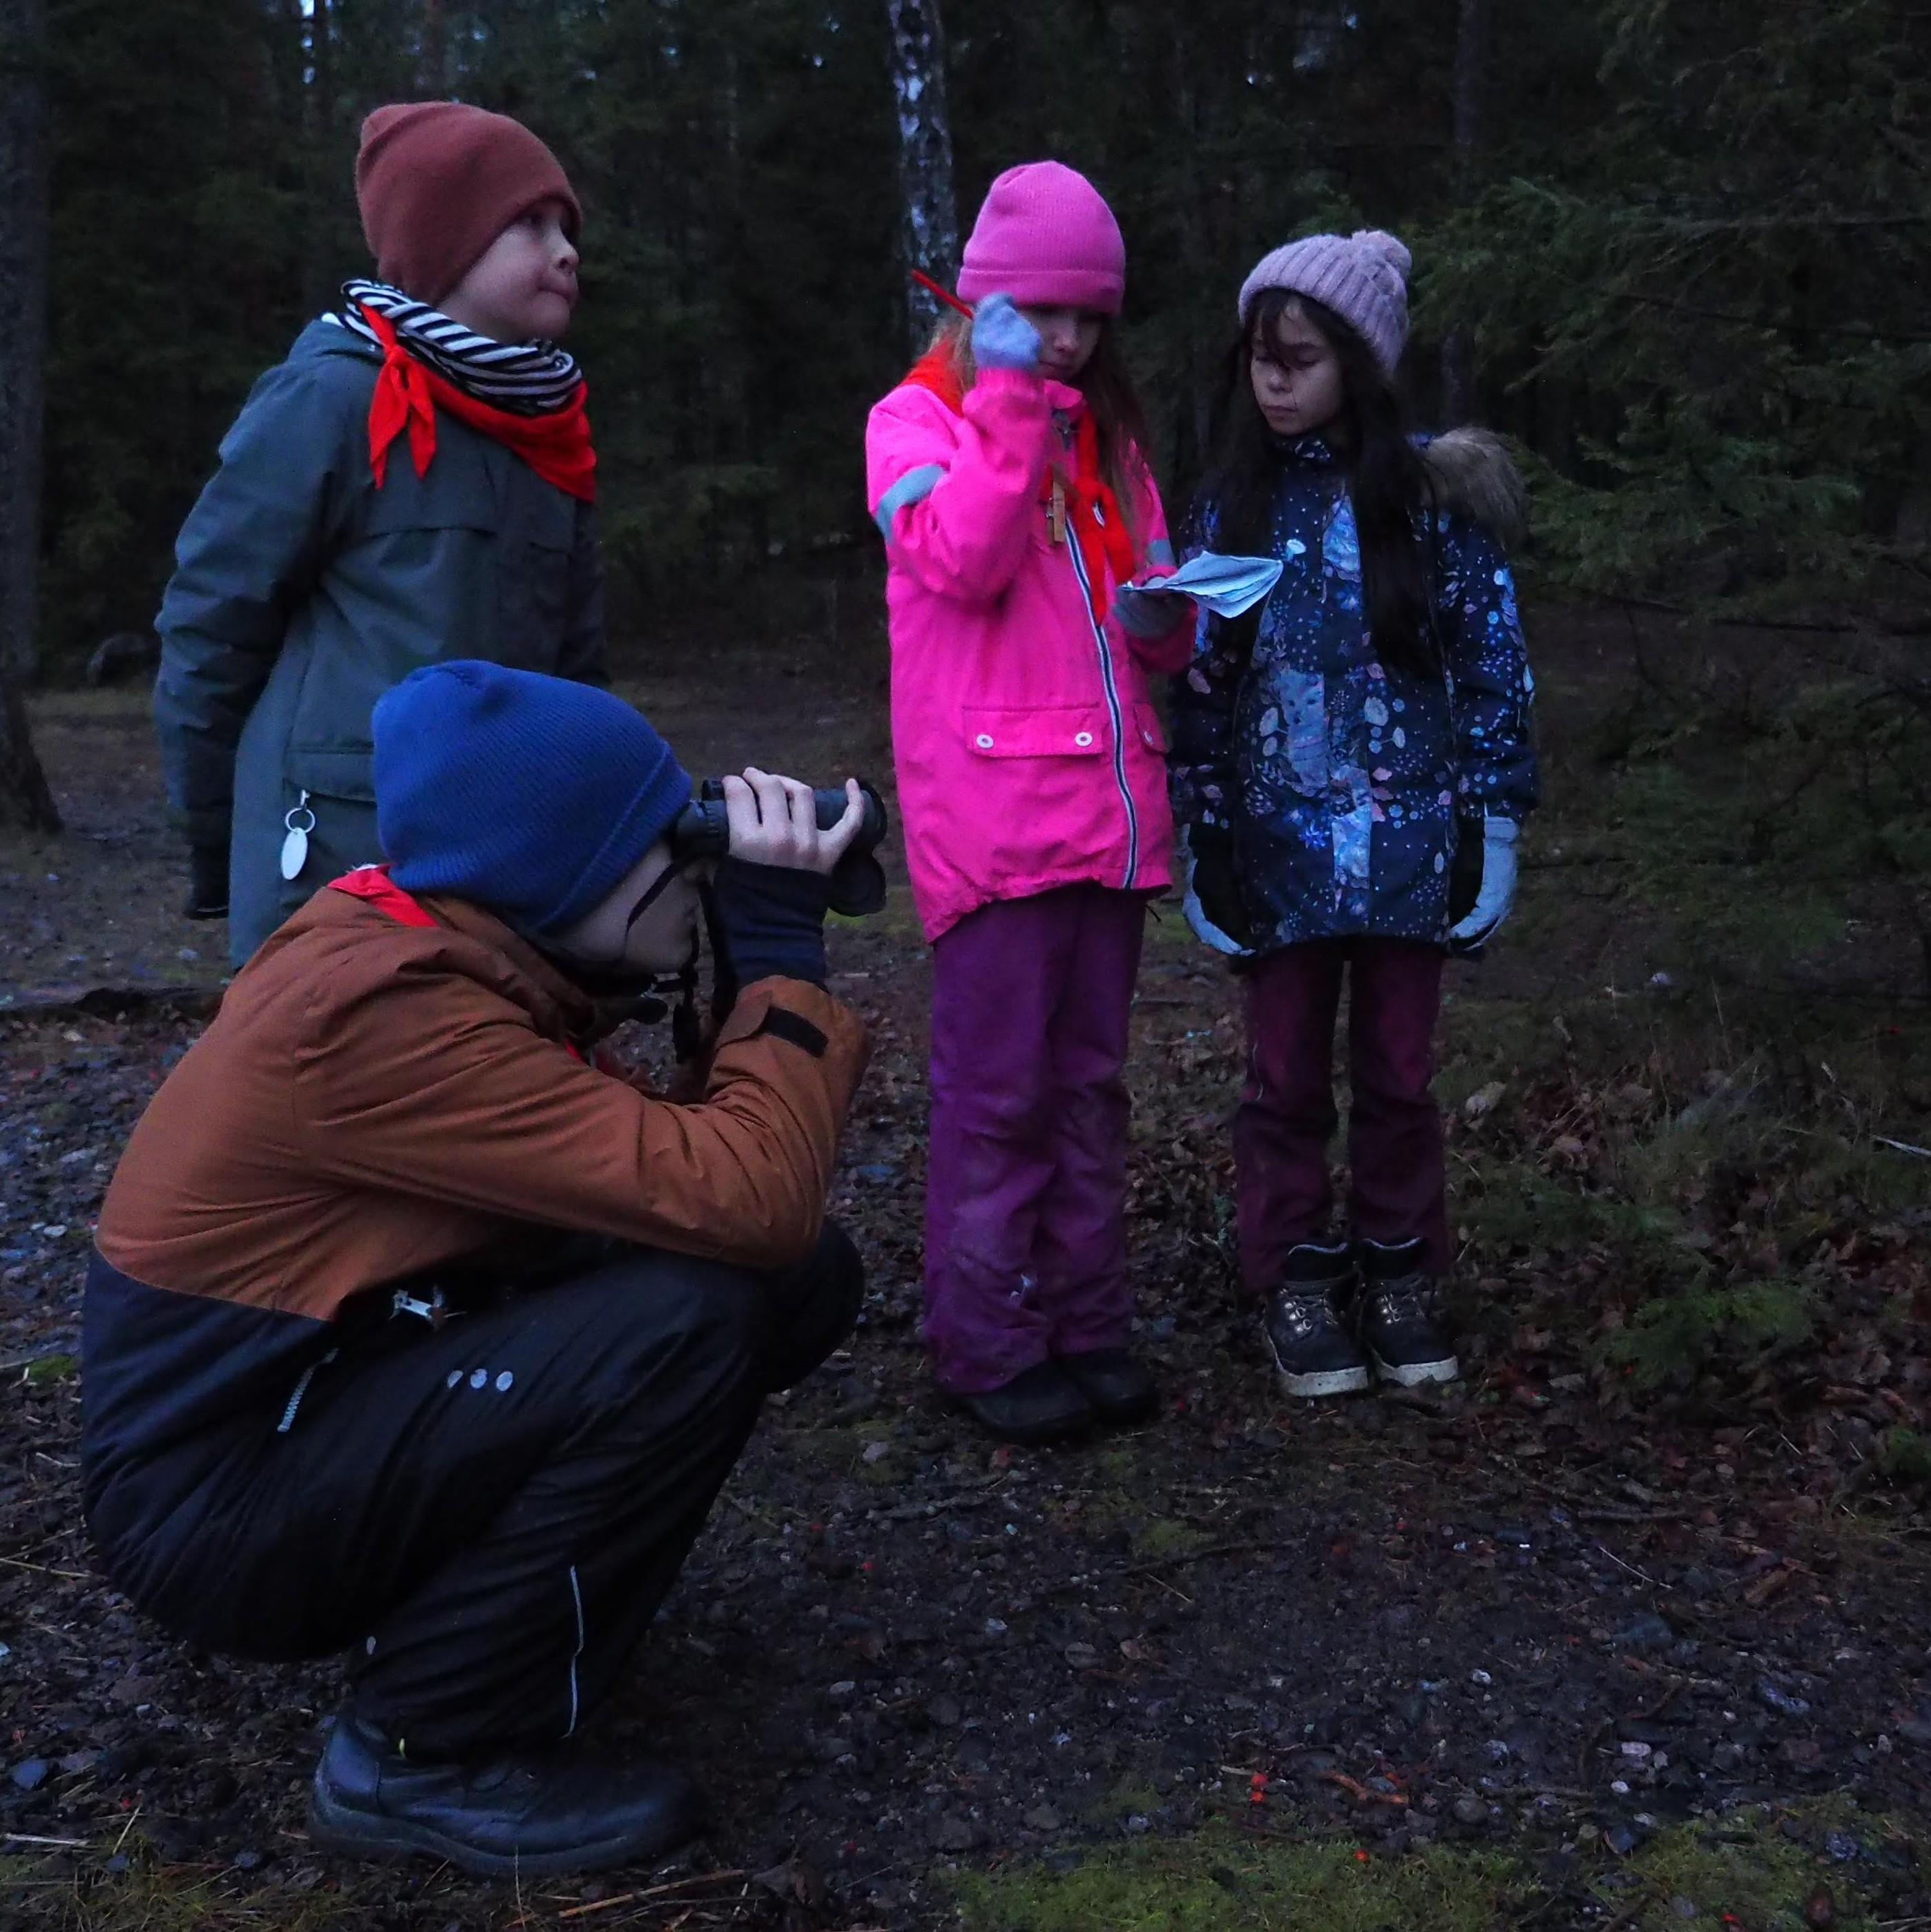
\includegraphics[width=.475\textwidth]{assets/meriharjuLinnut}
\caption{Neonvalo-vartio Kuusenalusmatto-rastilla ja Tyypit-vartio Poro, peura tai hirvi? -rastilla.}
\end{figure*}

Peräti 24 rusakkoa kokoontui jo tutuksi käyneellä bussilinja 560:n 
pysäkillä Kontulassa, josta matka jatkui kohti itää. Kävely Vuosaaren 
metroasemalta luontotalolle oli nuorempien retkeläisten mielestä 
jännittävä, kun viimeisellä kilometrillä ei ollutkaan enää 
katuvalaistusta. Tasku- ja otsalamput kaivettiinkin esiin hyvissä ajoin 
lyhyellä tauolla Sumujen sillalla. 

Kämpän pihalla vuorossa oli retkenjohtajan lyhyt ohjeistus ja Vene"-vartion 
leikkikimara ennen sisään siirtymistä ja majoittautumista: uniikki, 
sisäkissa"-ulkokissa ja lännen nopein. Kolkat yöpyisivät yhdessä 
huoneessa, seikkailijat ja tarpojat toisessa, samoajat ja Nonna kolmannessa ja 
muut johtajat neljännessä huoneessa. Retken kokonaisvahvuus oli 33 eli kaikki 
sänkypaikat paitsi yksi tulivat käytettyä.

Voileipäiltapalan jälkeen siirryttiinkin jo iltatoimille ja nukkumaan. Osa 
seikkailijoista ja tarpojista jäi vielä hetkeksi valvomaan takahuoneeseen ja 
osa johtajista kävi perjantaisaunassa.

Lauantaiaamu käynnistettiin kaurapuurolla ja pian oli aika suunnistukselle. 
Matkaan lähti viisi vartiota: Sudet, Neonvalo, Pupunkorvat, Tyypit ja 
S.U.P.E.R.G.A.L.A.K.T.I.S.E.T. F.E.M.I.N.I.S.T.I.M.A.R.S.U.T. (lyhyemmin 
S.G.F.M.). Rastikiertoon liittyi retken teemaan sopiva kehystarina, joka 
mukaili Marketta Pyysalon kertomusta \textit{Siili, jonka joulu herätti}. 

Suunistuksen ensimmäisellä rasteilla tunnistettiin eläinten lumijälkiä. 
Valitettavasti retkilauantaina ei vielä lunta maassa ollut, minkä vuoksi 
jälkien tunnistus tapahtui puhelimen näytöltä. Toisella rastilla vartion 
tehtävänä oli edetä pressun päällä rastihenkilön määräämä matka ja 
kolmannella laulaa joululauluja, joissa esiintyi tiettyjä sanoja. Neljäs 
rasti sijaitsi Niemenapajalla, jossa vartio etsi kertakäyttölusikoita 
maastosta.

\begin{figure*}[!t]
\centering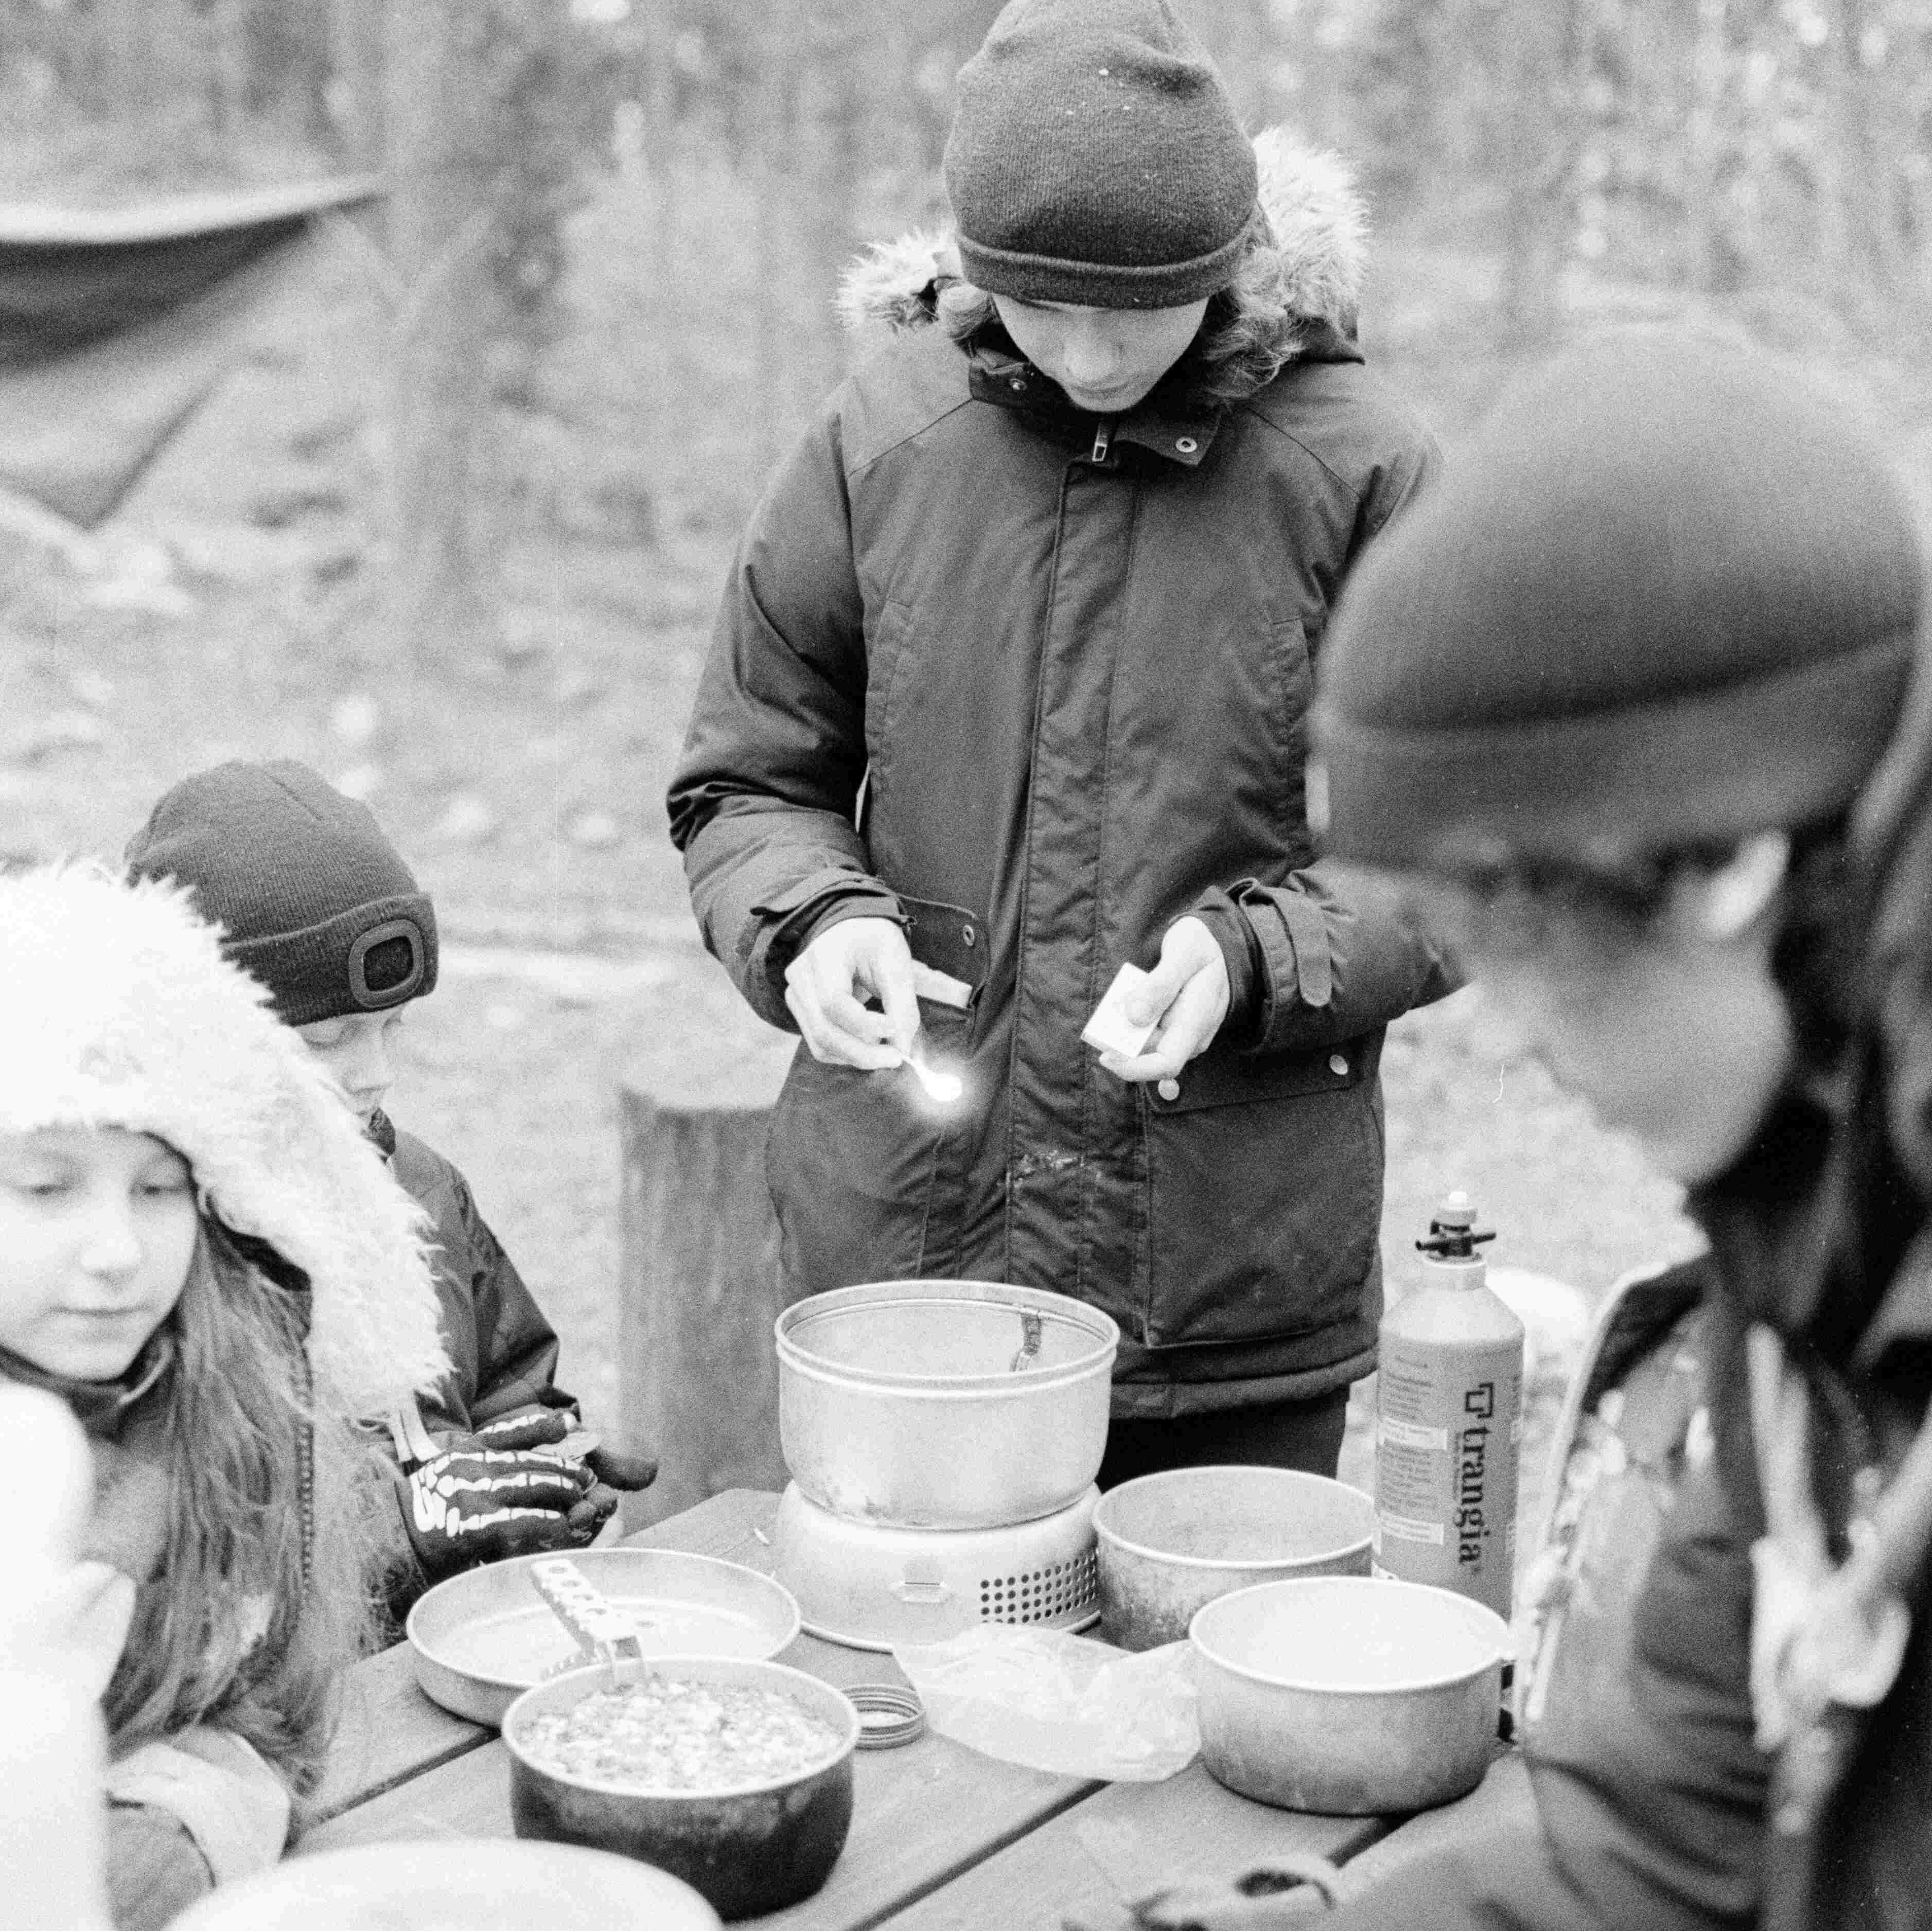
\includegraphics[width=.475\textwidth]{assets/meriharjuRuoka1}\hfill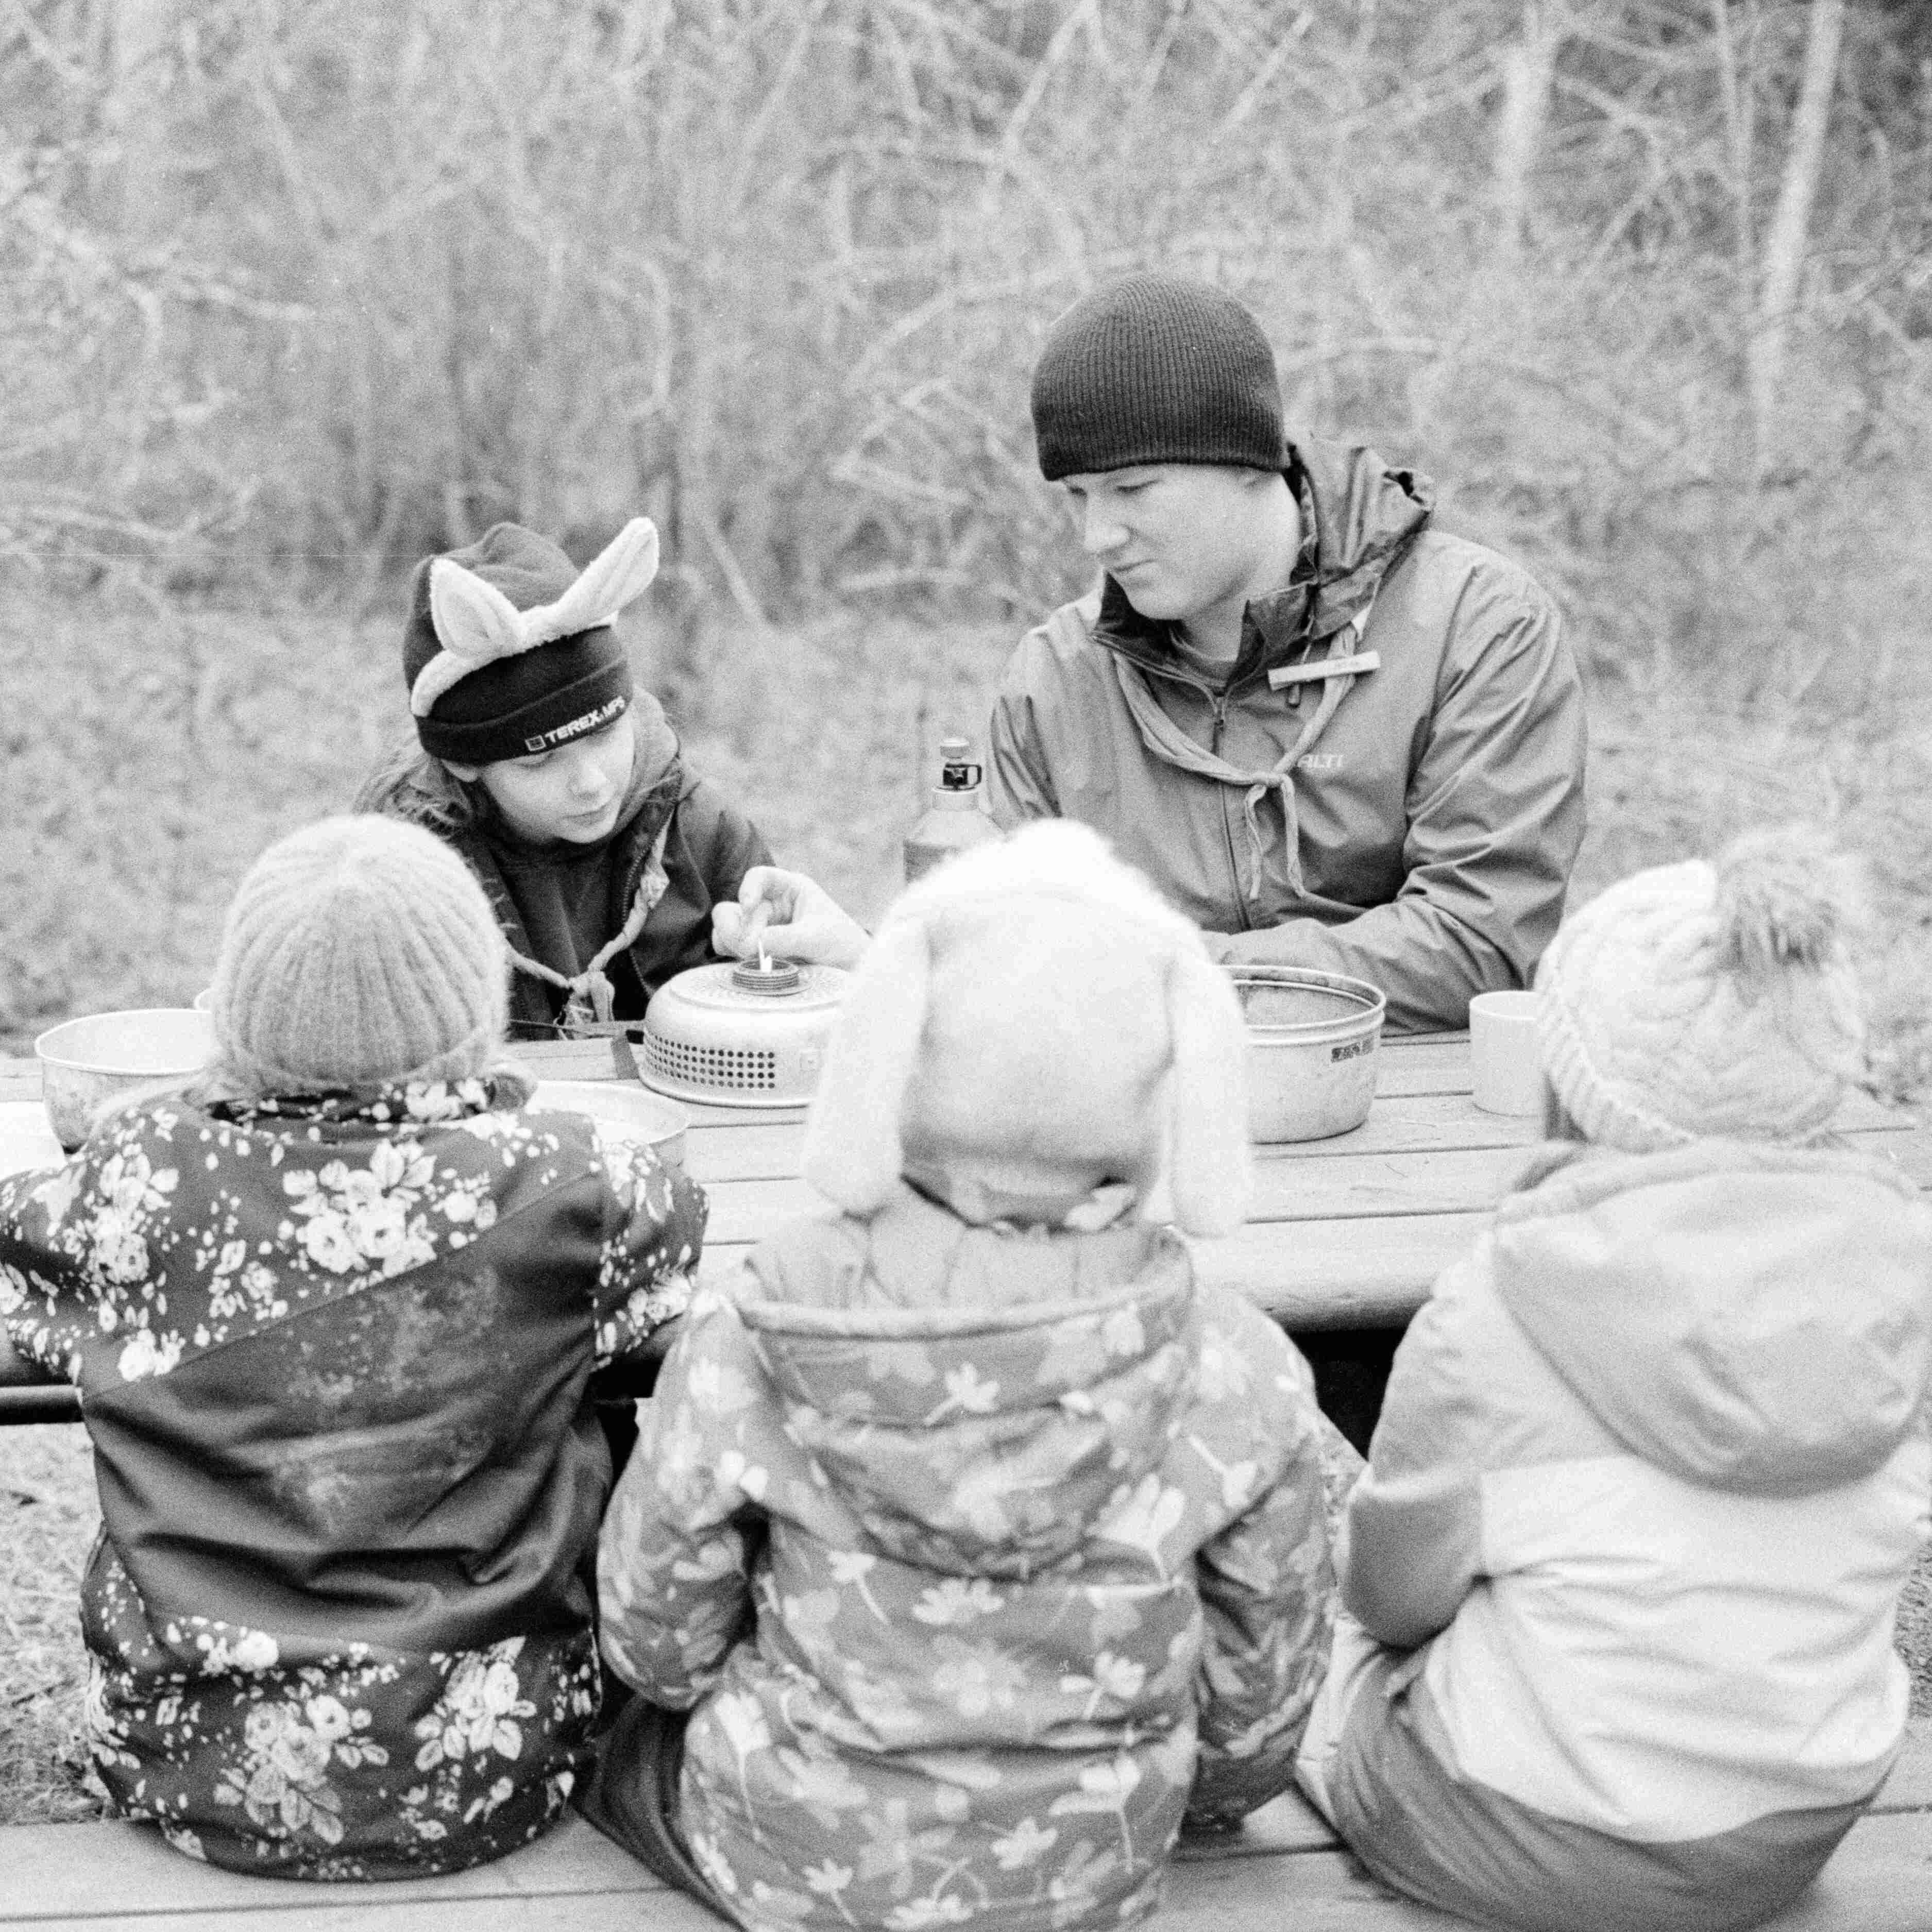
\includegraphics[width=.475\textwidth]{assets/meriharjuRuoka2}
\caption{Sudet- ja Pupunkorvat -vartiot ruokarastilla.}
\end{figure*}

Vielä oli kaksi rastia jäljellä, mutta ennen niitä vartiot valmistivat 
itselleen maittavan trangialounaan: tonnikalanuudeleita, nams! Tässä 
vaiheessa alkoi sataa vähän räntää, mutta se ei vartoiden menoa haitannut. 
Kuudennella rastilla tehtiin iso merimiessolmu ja seitsemännellä rastilla 
tunnistettiin eläimiä. Maalitehtävä oli muita rastitehtäviä huomattavasti 
haastavampi, kun vartioiden piti yhdistää maakunnan vaakuna sitä vastaavaan 
maakuntamaaeläimeen, "=lintuun tai "=kalaan. 

Vaikka varsinaisia suunnistuksia ei viime lippukuntaretkillä ole ollutkaan 
ohjelmassa, kaikki vartiot löysivät hienosti kaikille rasteille. Seitsemän 
rastin, vajaan kahdeksan kilometrin suunnistukseen meni nopeimmalta vartiolta 
noin viisi tuntia ja hitaimmalta kuusi tuntia. Nopeudesta ei saanut pisteitä, 
mutta rastitehtävät pisteytettiin -- löydät vartoiden pisteytykset 
jutun lopun taulukosta. Onneksi olkoon, Tyypit!

Samaa vauhtia kuin vartiot saapuivat suunnistuksen maaliin vartiot alkoivat 
suunnitella omia piparkakkutalojaan. Kukin vartio sai käyttöönsä kokonaisen 
kilon piparkakkutaikinaa, josta tarkoituksena oli rakentaan kullekin vartiolle 
mieluisa teos. Varsin moni vartio rakensi perinteikästä piparkakkutaloa 
mukailevan rakennelman, mutta myös jännittävämpiä ratkaisuja kuten 
piparkakkunelitahokas ja piparkakkupelikortit nähtiin. Myös teokset 
pisteytettiin.

\begin{figure*}[!t]
\centering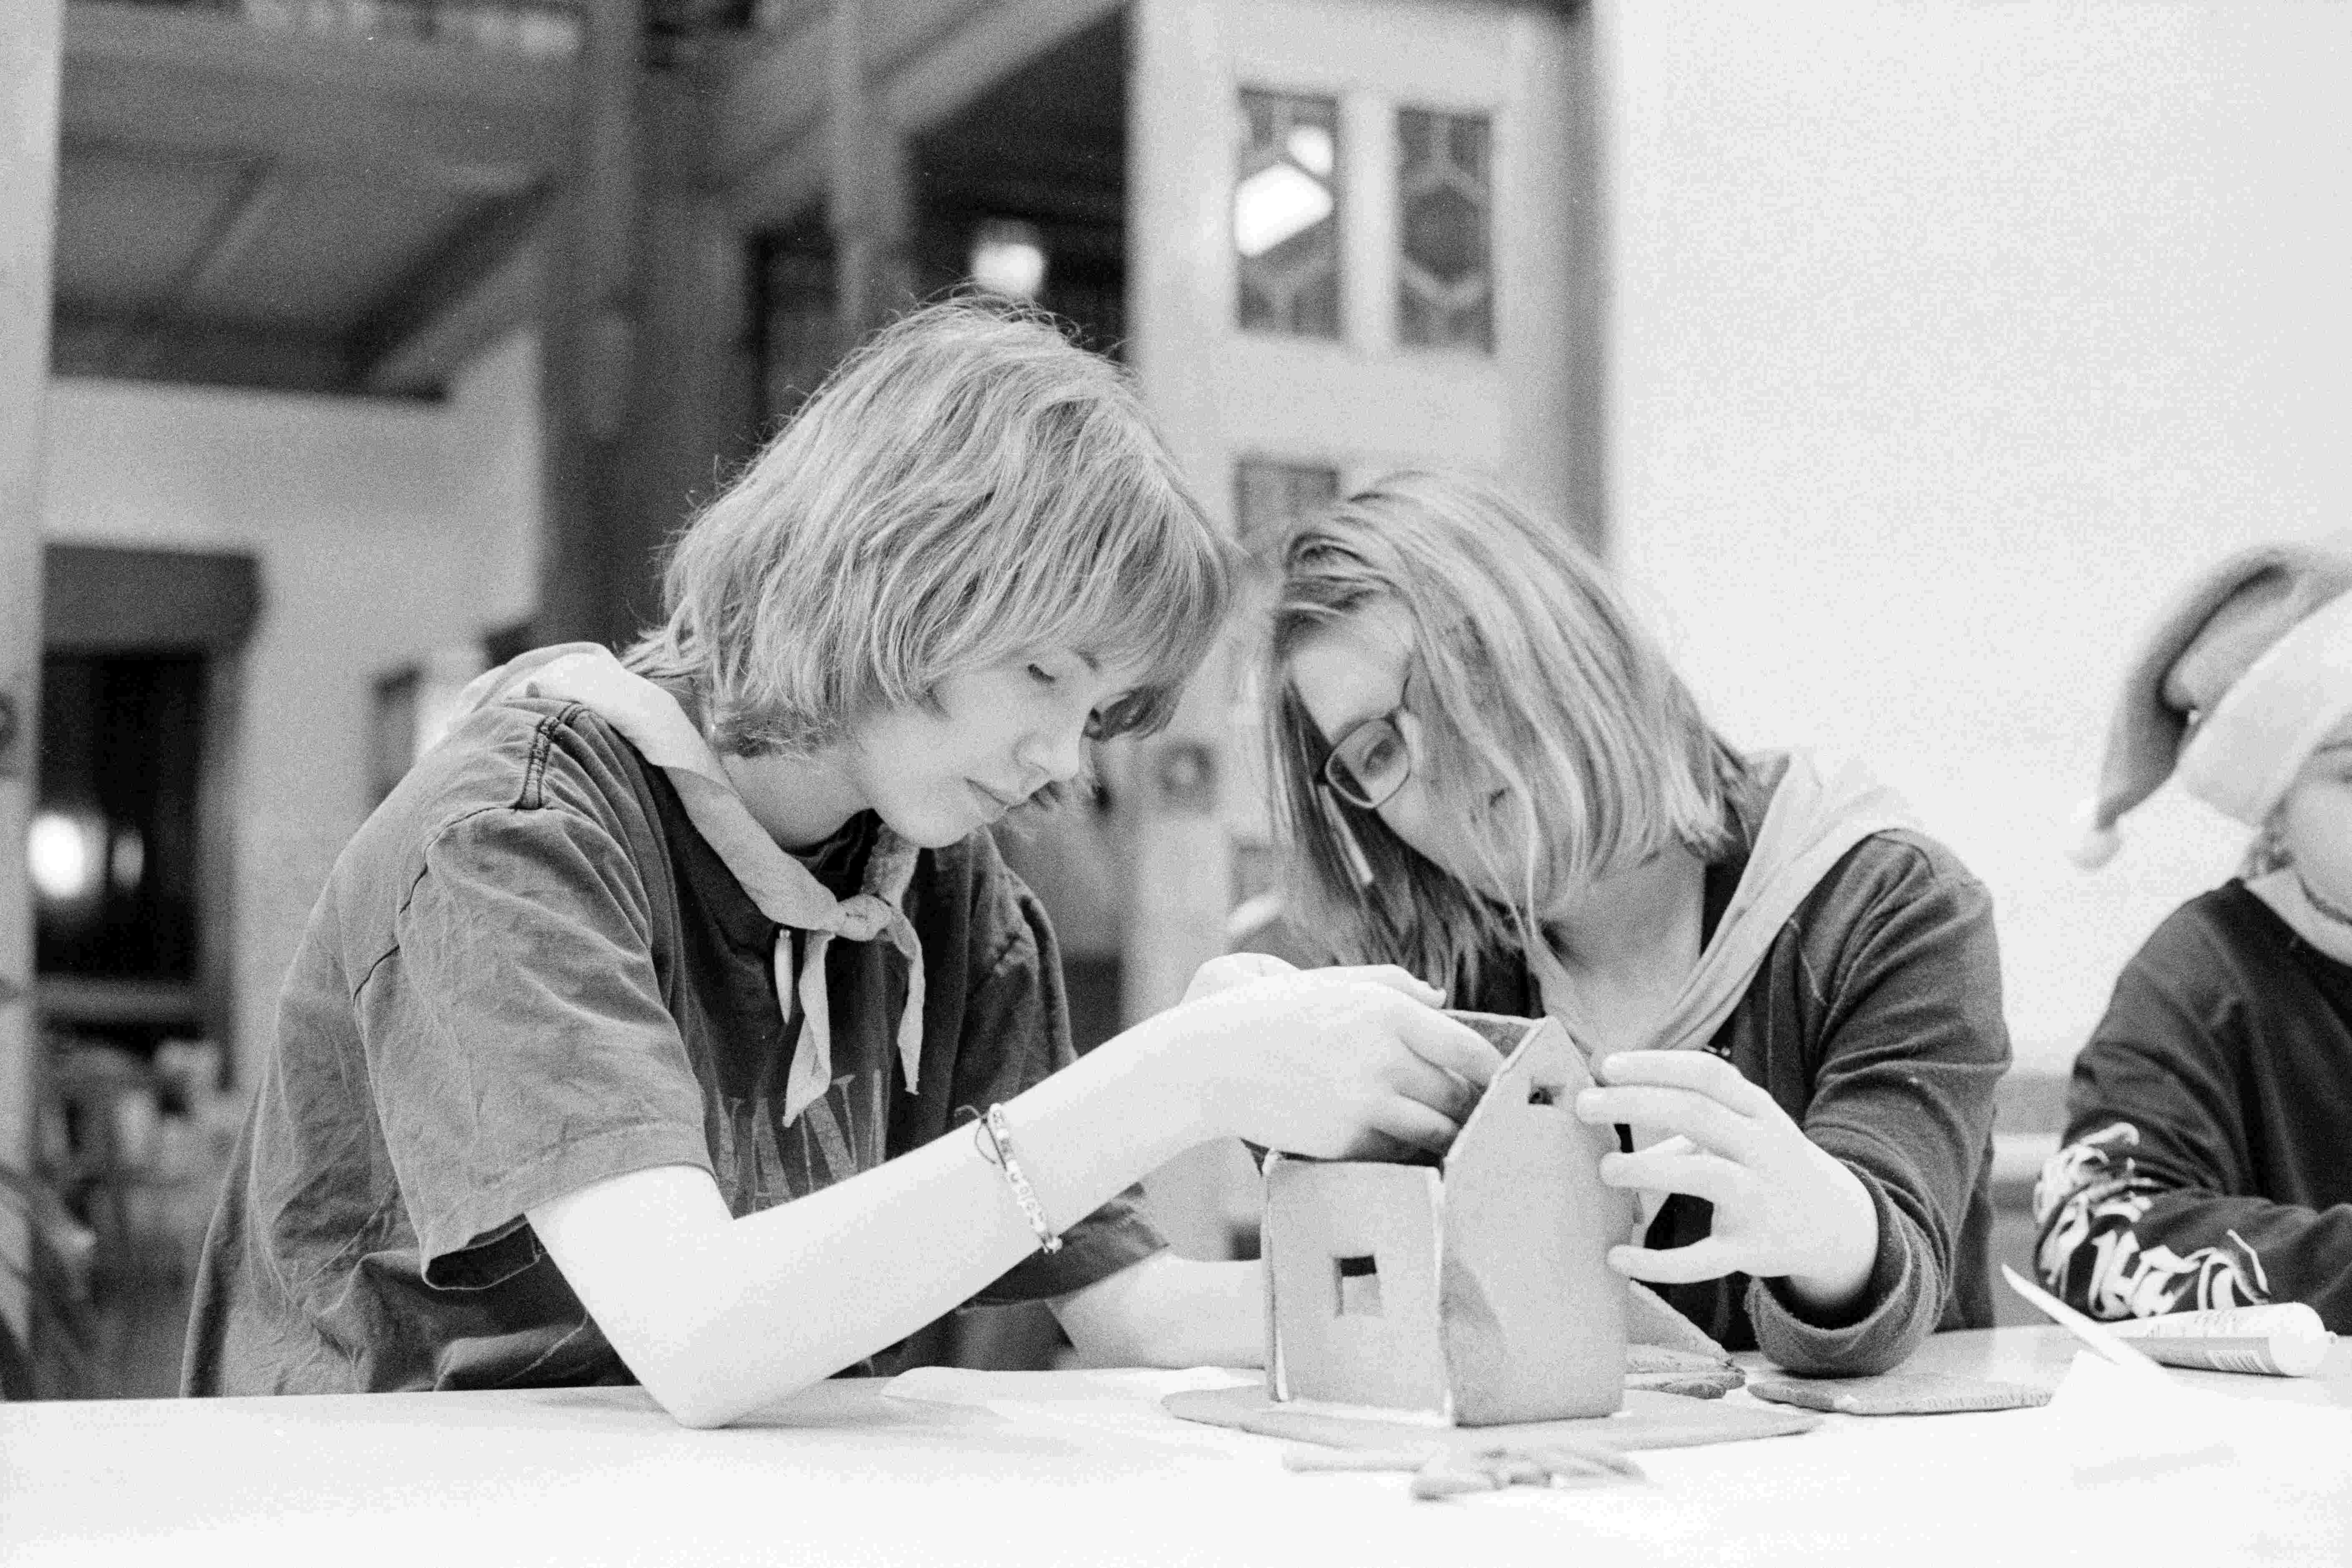
\includegraphics[width=\textwidth,trim={0 0 0 5cm},clip]{assets/meriharjuPipari}
\caption{S.U.P.E.R.G.A.L.A.K.T.I.S.E.T. F.E.M.I.N.I.S.T.I.M.A.R.S.U.T. -vartio rakentamassa piparkakkutaloa.}
\end{figure*}

\begin{table*}[b]\centering\small
\begin{tabular}{|l|c|c|c|c|c|}
\hline
 & \textbf{Tyypit} & 
\begin{tabular}[x]{@{}c@{}}\textbf{Pupun-}\\\textbf{korvat}\end{tabular} & 
\begin{tabular}[x]{@{}c@{}}\textbf{Neon-}\\\textbf{valo}\end{tabular} & 
\textbf{Sudet} & \textbf{S.G.F.M.} \\ \hline
\textbf{Lumijälkiä} & 3,00 & 3,00 & 1,00 & 3,00 & 5,00 \\ \hline
\textbf{Kuusenalusmatto} & 13,12 & 12,14 & 11,82 & 11,46 & 0,00 \\ \hline
\textbf{Kauneimmat joululaulut} & 10,00 & 8,00 & 7,00 & 2,00 & 6,00 \\ \hline
\begin{tabular}[x]{@{}c@{}}\textbf{Pata-himmeli 
ja}\\\textbf{ruutu-kranssi}\end{tabular} & 3,00 & 5,00 & 3,00 & 4,00 & 5,00 \\ 
\hline
\textbf{Joulurusetti} & 5,00 & 5,00 & 4,00 & 4,00 & 5,00 \\ \hline
\textbf{Poro, peura tai hirvi?} & 4,00 & 6,00 & 3,00 & 5,50 & 3,00 \\ \hline
\textbf{Joulun taikaa} & 25,00 & 12,50 & 25,00 & 12,50 & 12,50 \\ \hline
\textbf{Piparkakkutalot} & 30,00 & 35,00 & 24,00 & 35,00 & 37,00 \\ \hline \hline
 & 93,12 & 86,64 & 78,82 & 77,46 & 73,50 \\ \hline
\end{tabular}
\end{table*}

Piparkakkuteosten osien paistuessa syötiin herkullista kanapataa. 
Päivällisen jälkeen halukkaat kävivät saunomassa muiden laulaessa 
joululauluja ja koristellessa teoksiaan. Iltapalaksi oli jotain hieman 
erikoisempaa: nyhtöleipää, keksejä ja paukkumaissia!

Sunnuntaiaamu käytettiin pakkaamiseen ja siivoamiseen. Uusille kolkille 
järjestettiin kolkkakoe, jonka kaikki kolme kokelasta läpäisivät. Lounaaksi 
juuri ennen joulujuhlaa syötiin riisipuuroa. 

\begin{figure*}[p]
\centering
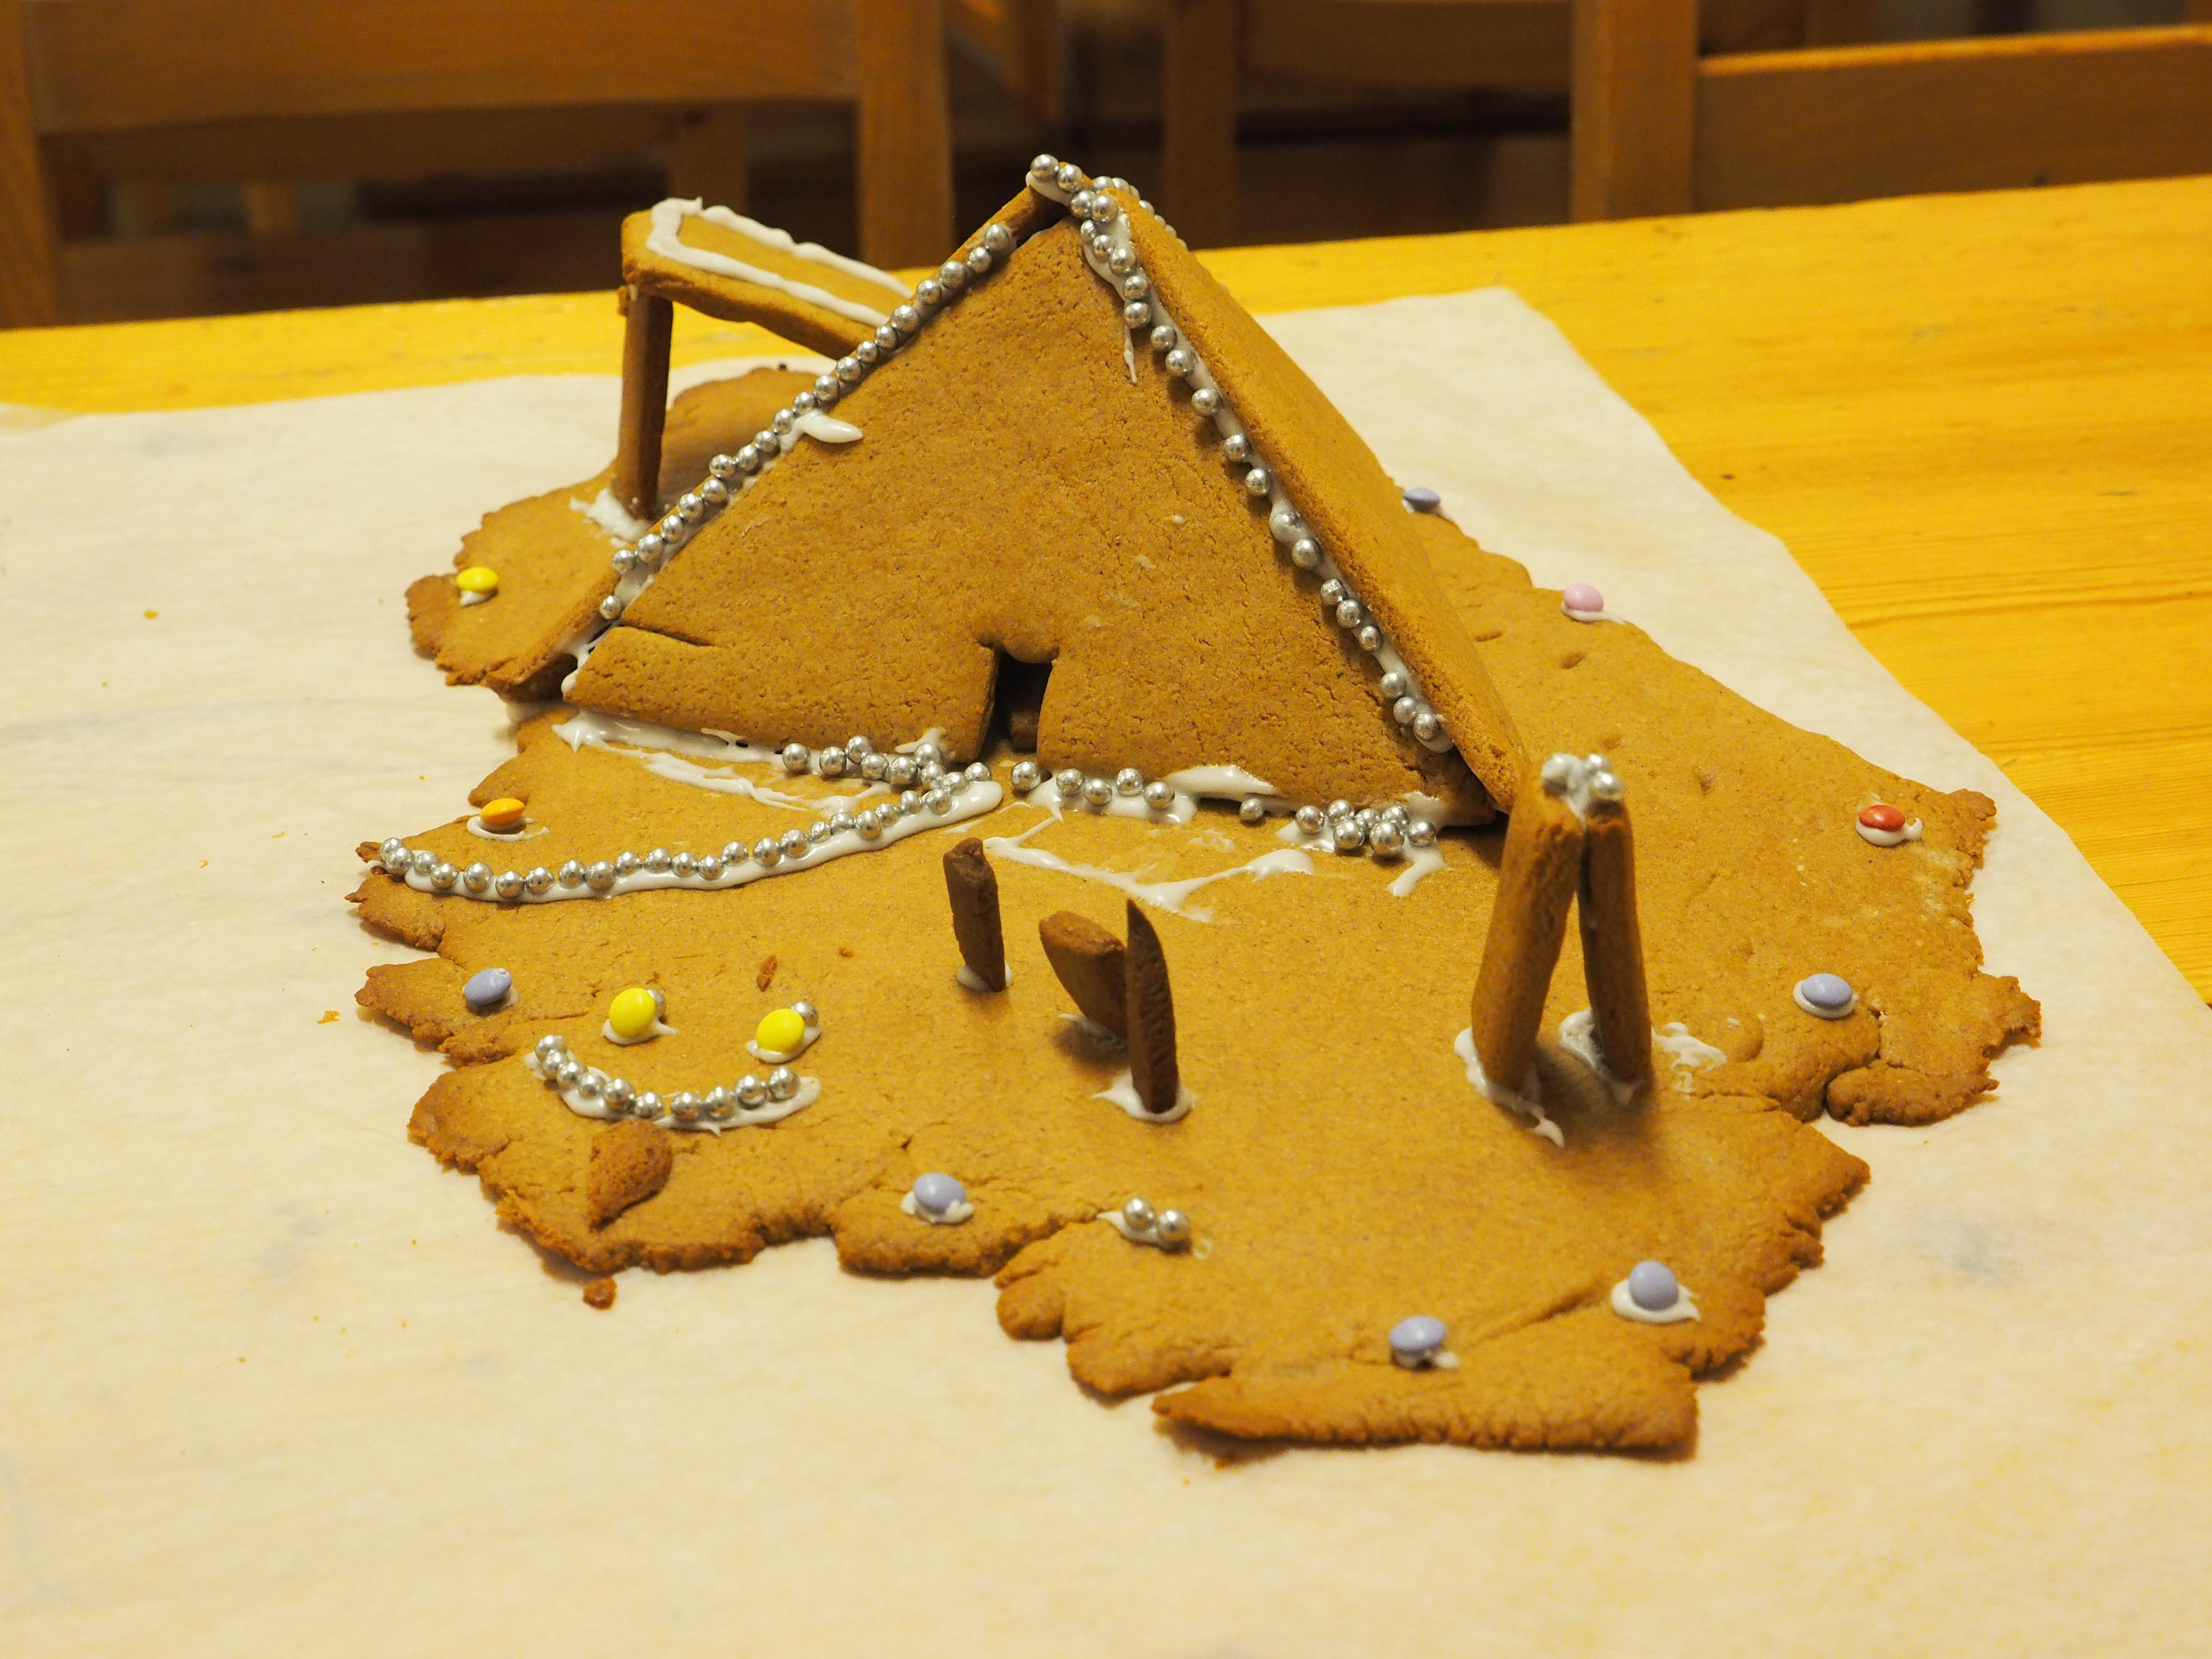
\includegraphics[width=.475\textwidth,height=.475\textwidth,keepaspectratio]{assets/pipari1}\hfill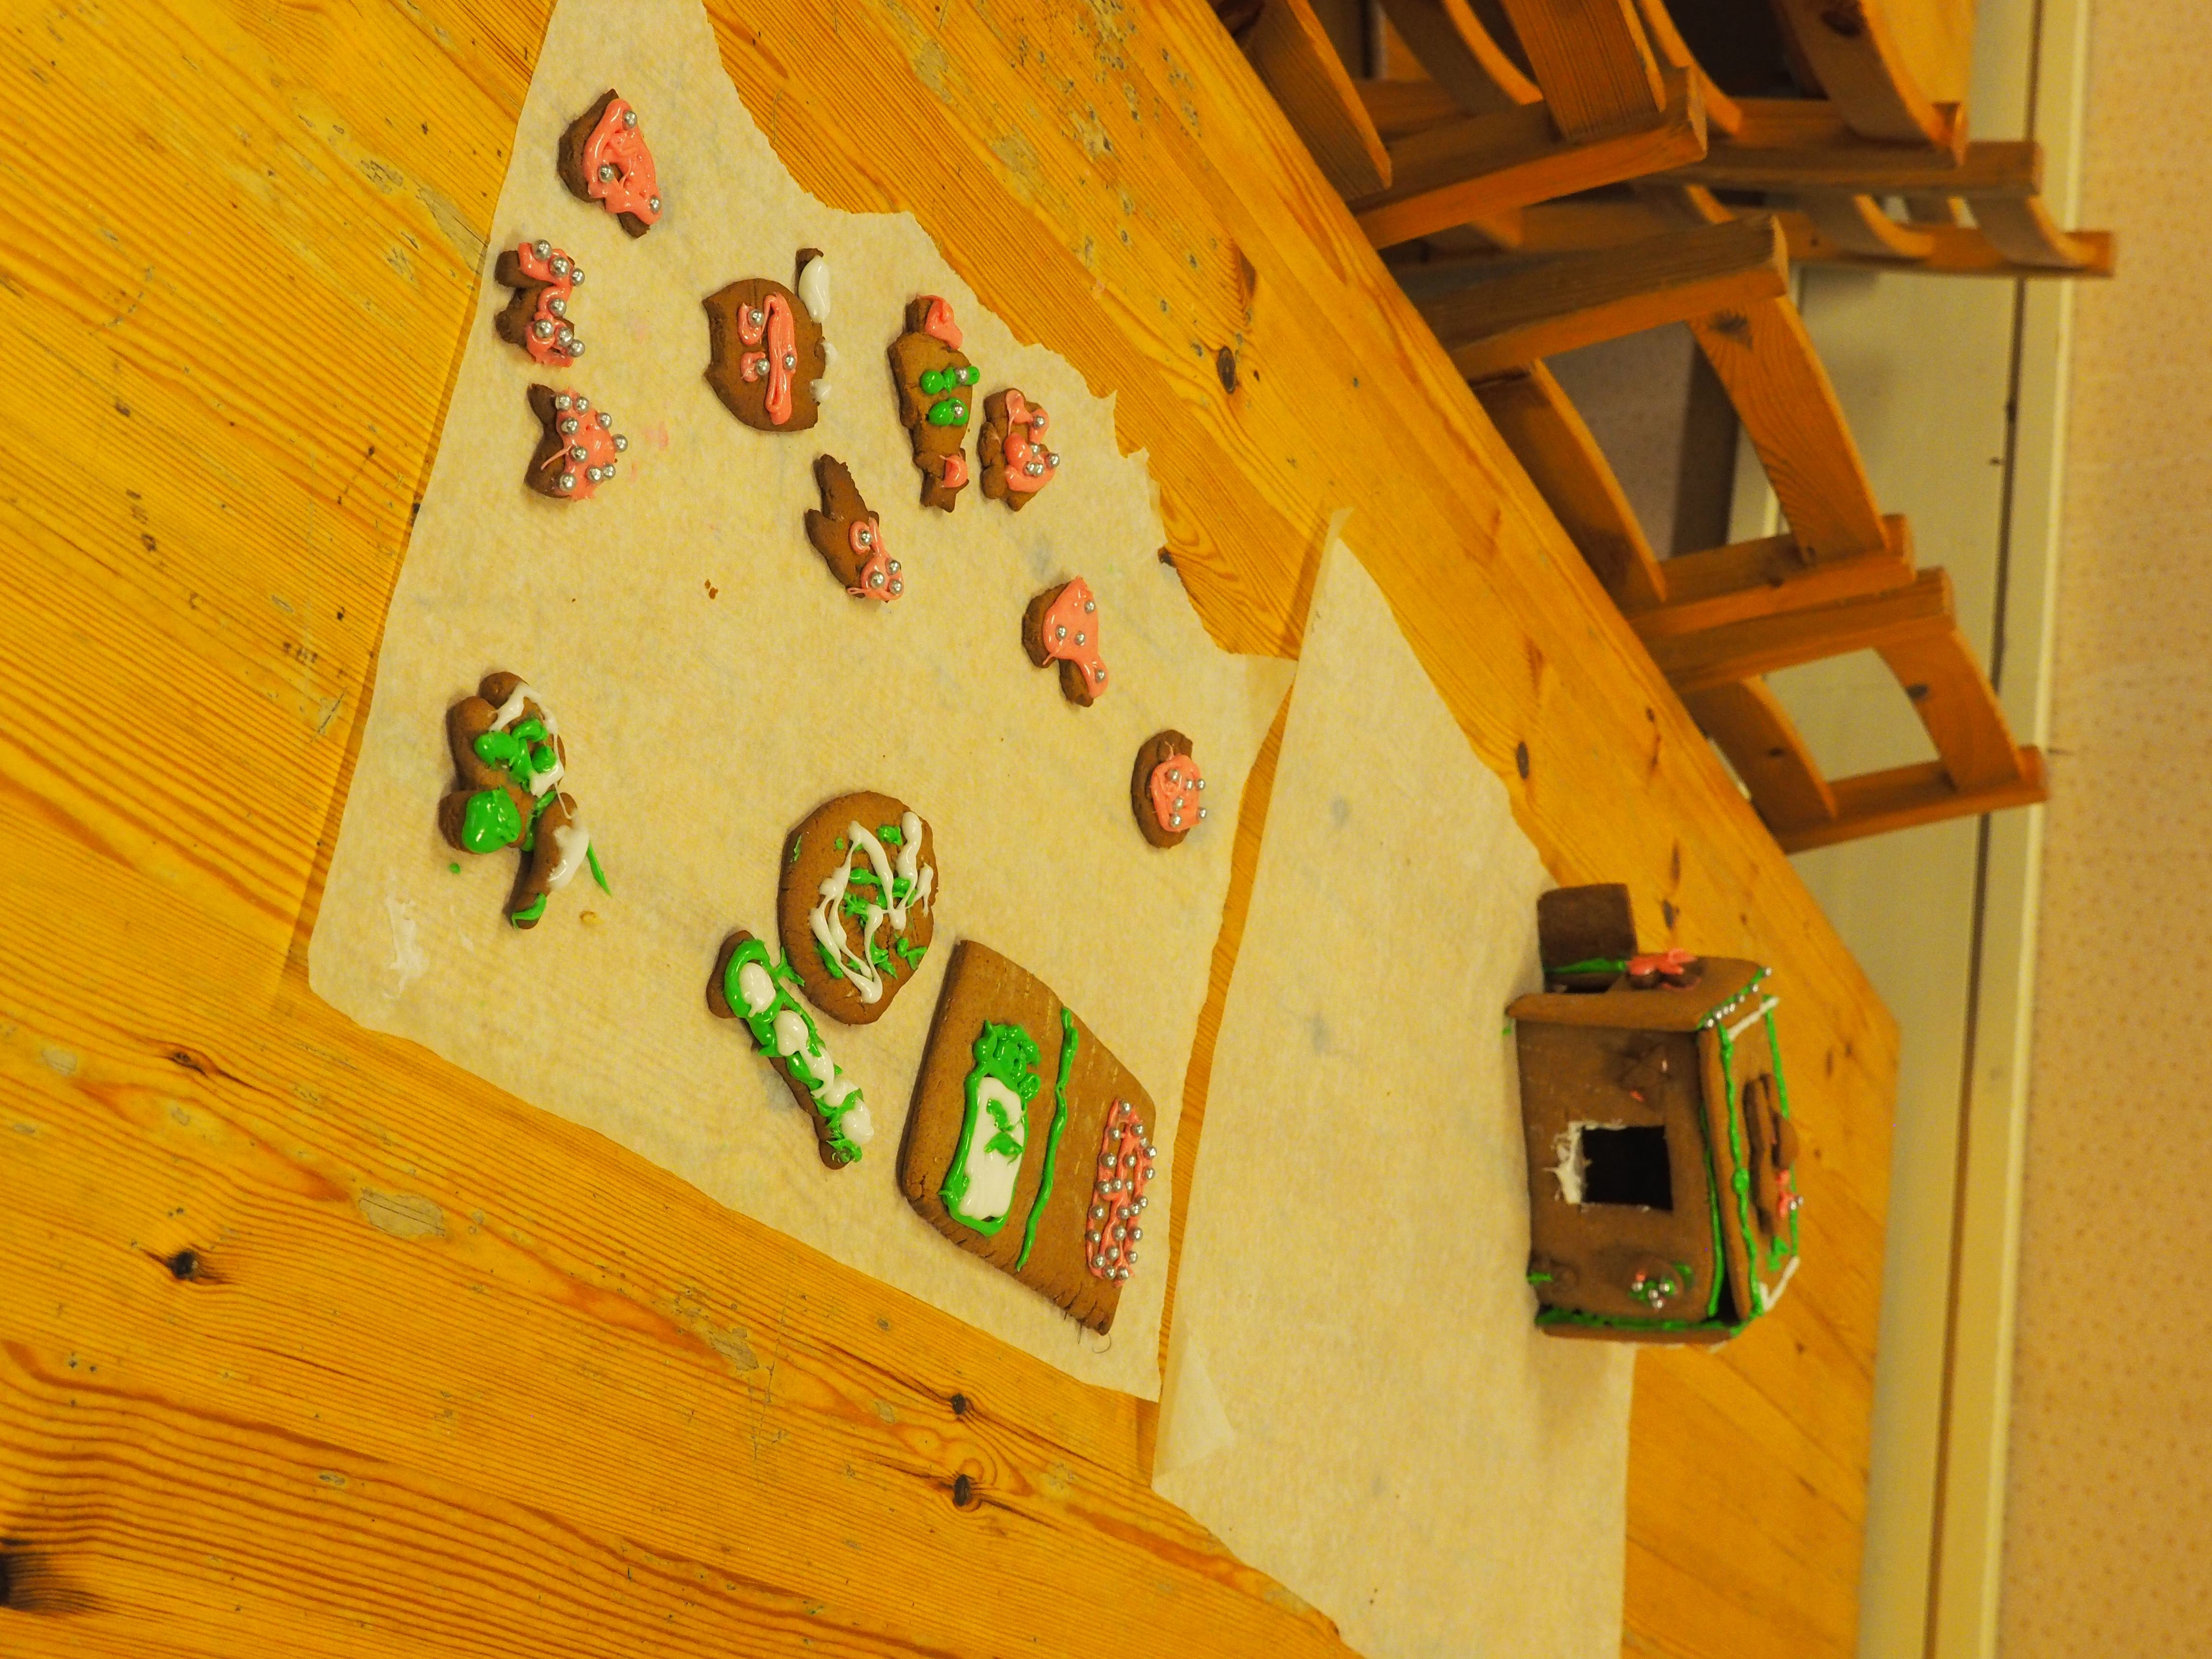
\includegraphics[width=.475\textwidth,height=.475\textwidth,keepaspectratio,angle=90]{assets/pipari2}

\vspace*{.05\textwidth}

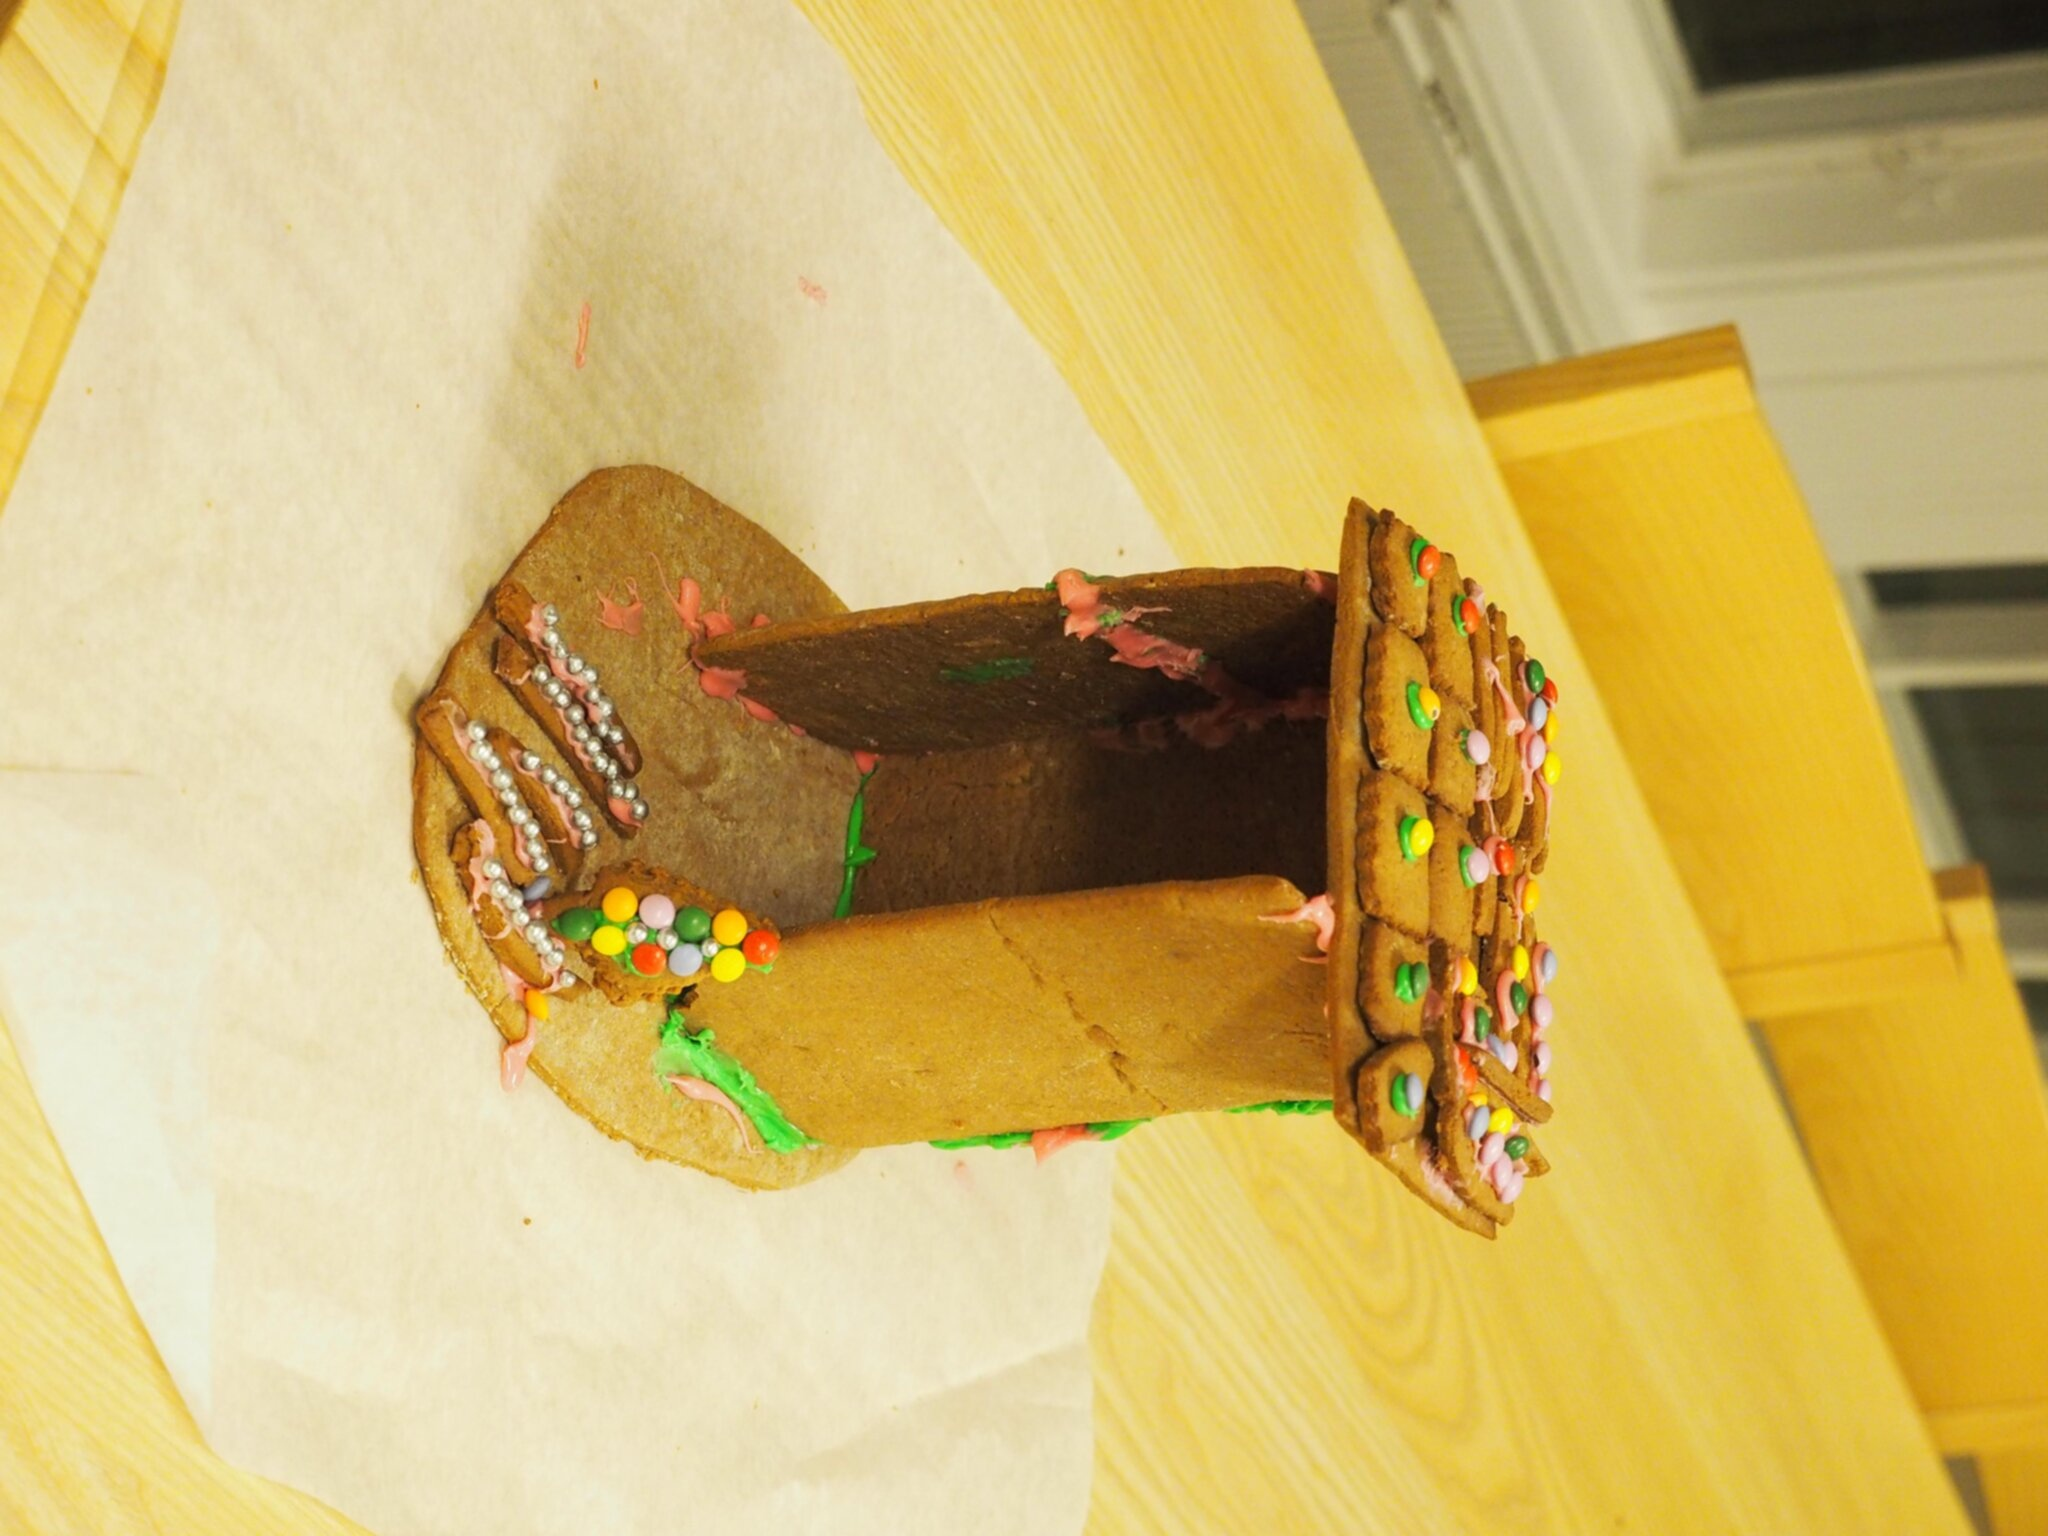
\includegraphics[width=.475\textwidth,height=.475\textwidth,keepaspectratio,angle=90]{assets/pipari4}\hfill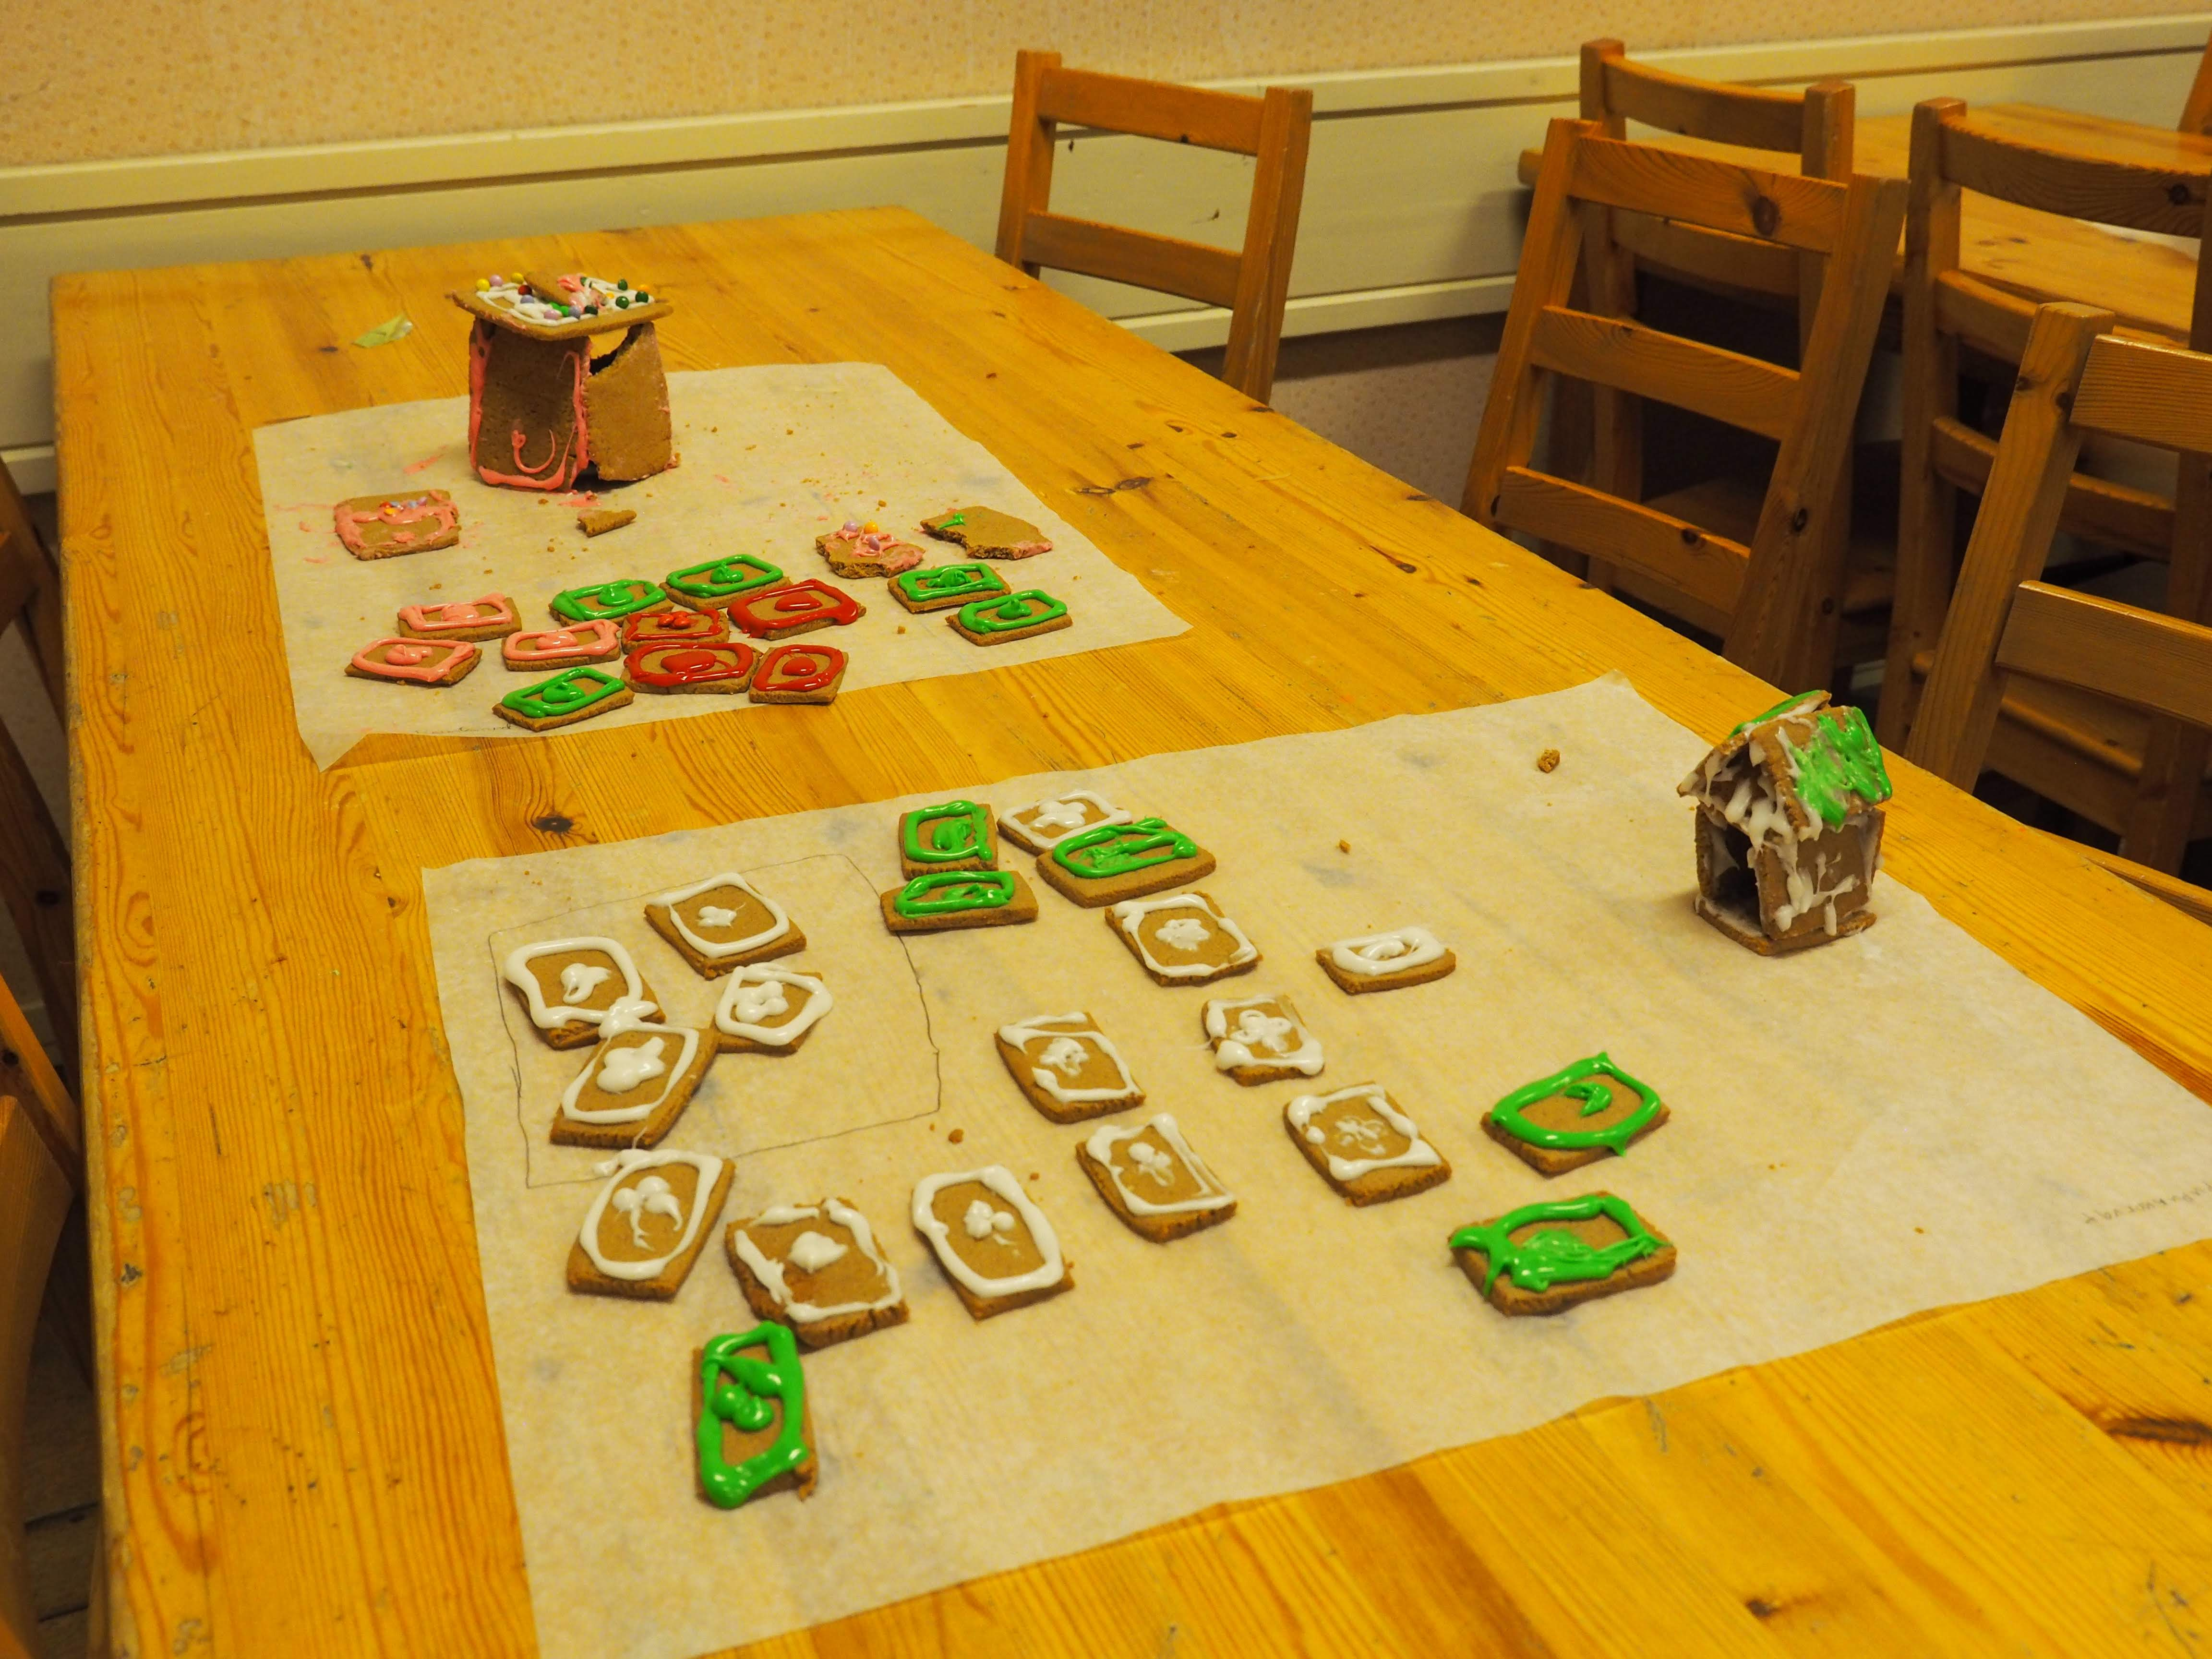
\includegraphics[width=.475\textwidth,height=.475\textwidth,keepaspectratio]{assets/pipari3}

\vspace*{.05\textwidth}

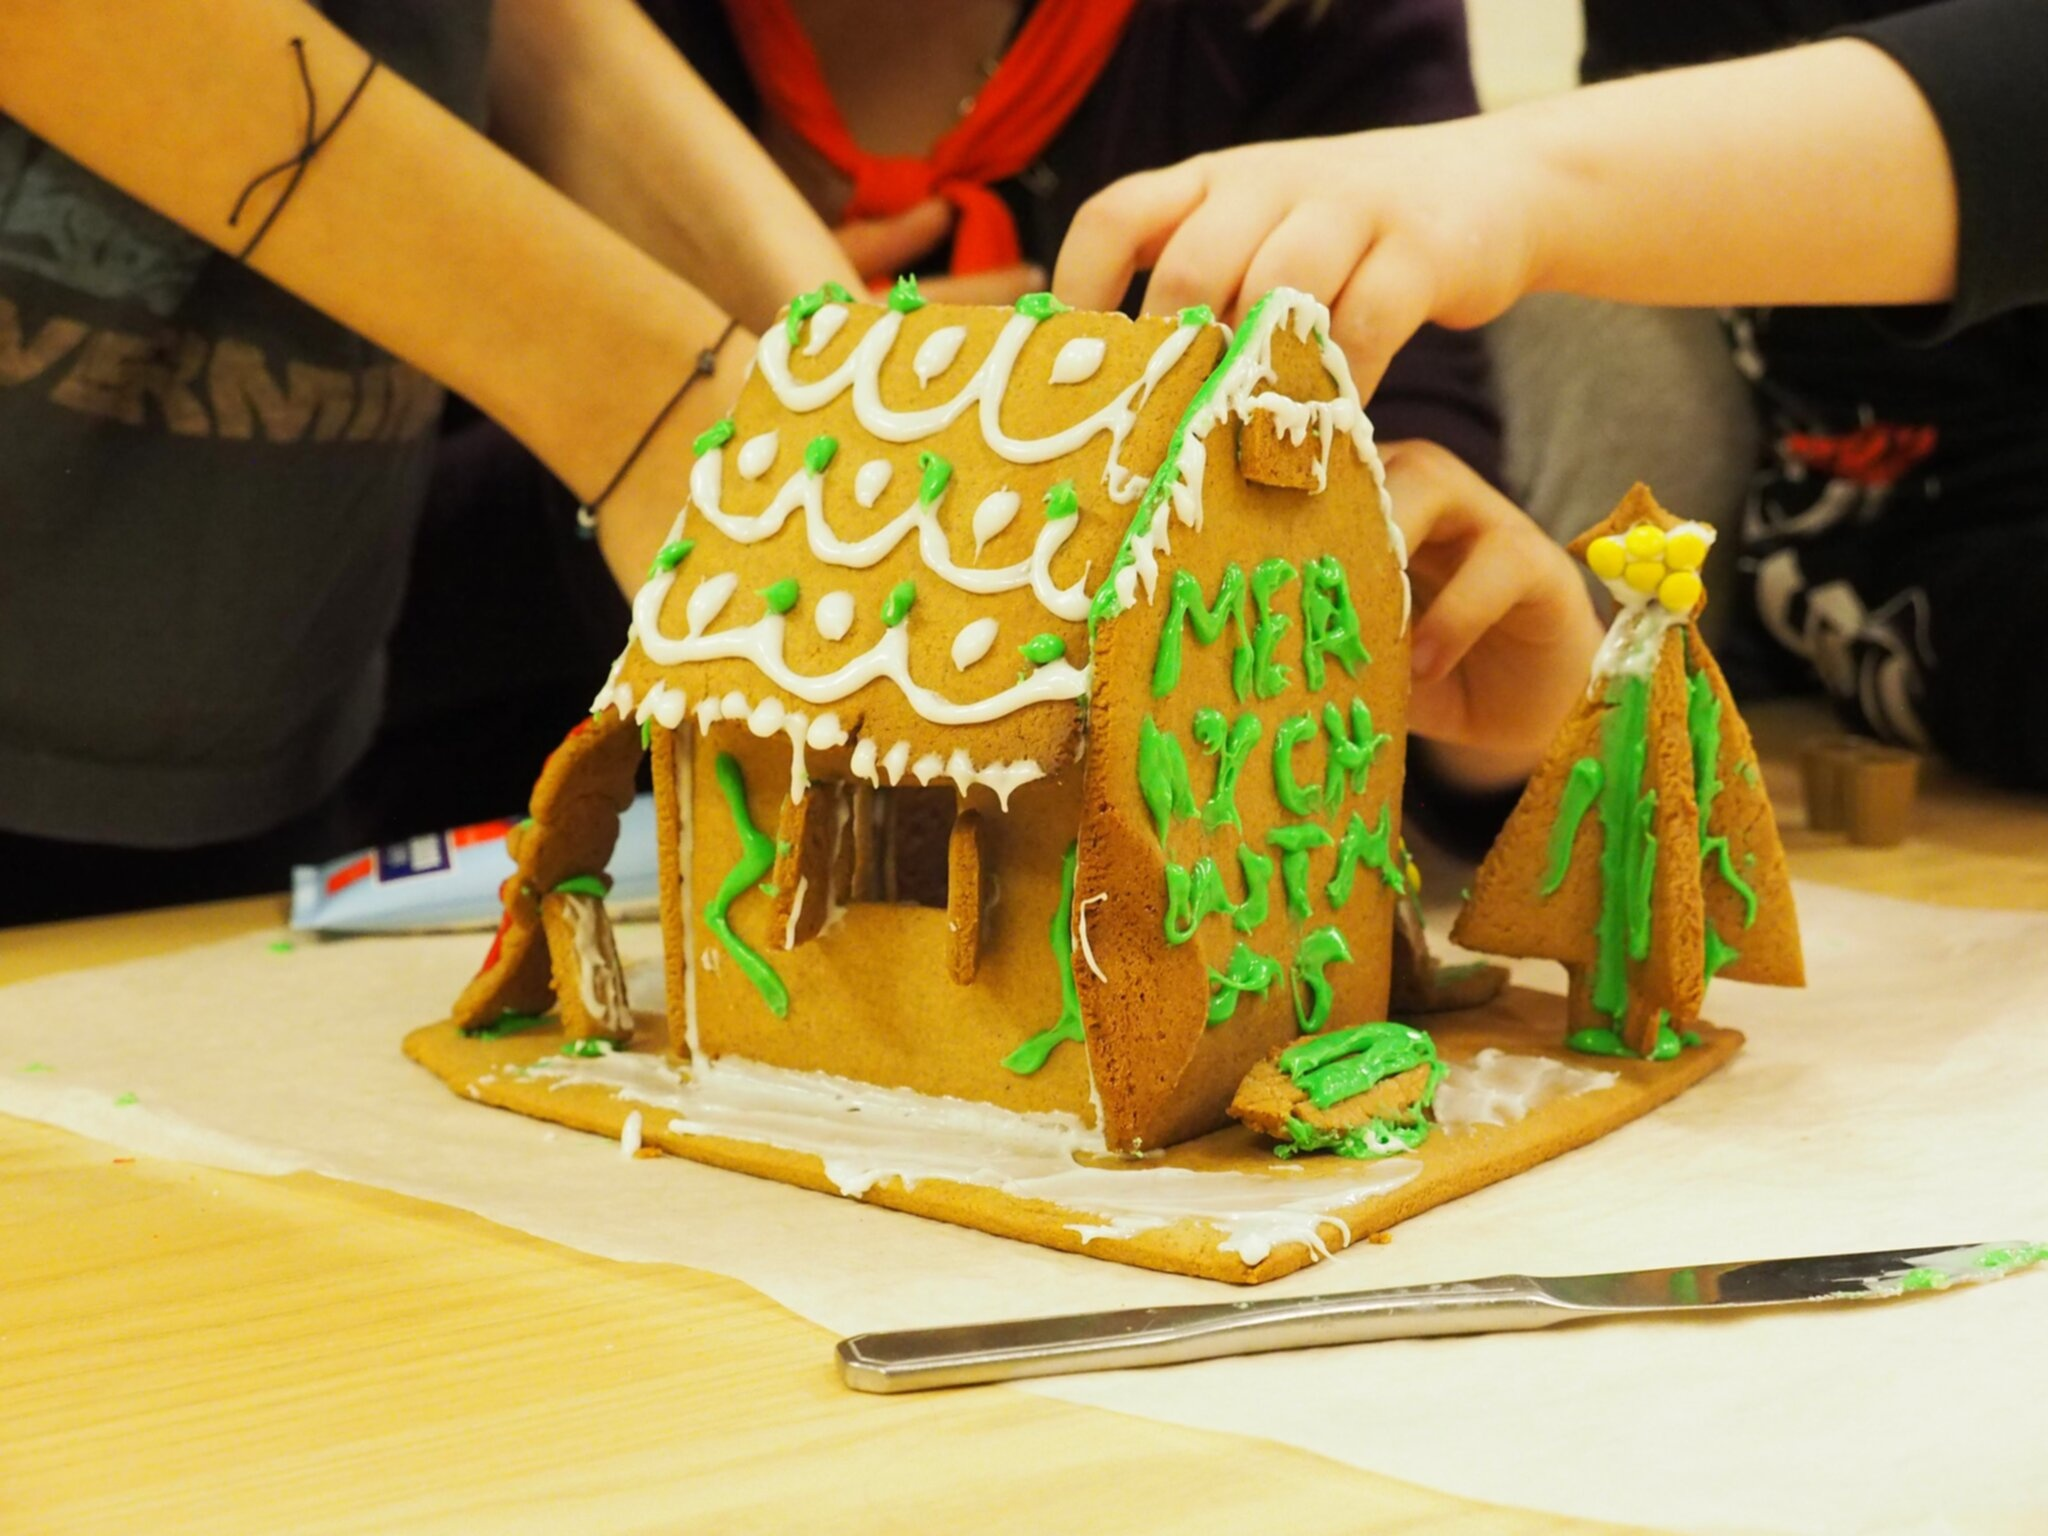
\includegraphics[width=.475\textwidth,height=.475\textwidth,keepaspectratio]{assets/pipari5}

\caption{Vartioiden piparkakkuteokset.}
\end{figure*}

Joulujuhlan juonsivat Tesla ja Touko ja se alkoi Päärynähyttysten 
spektaakkelimaisella näytelmällä joulupukista, tountuista ja nuuttipukista, 
joka huipentui joulupukin ja nuuttipukin eeppiseen räppäyskilpailuun! Listan 
joulujuhlassa ansioituneista löydät edellisestä Tassusta.

Juhlan päätyttyä luontotalo siivottiin loppuun ja lähdettiin kotimatkalle. 
Mitäköhän keksimmekään taas tämän vuoden pikkujouluretkelle?
\end{multicols}

\medskip

\noindent\null\hfill Kuvat: Janne ja Tanguy\\
\noindent\null\hfill Teksti: Janne


% 
\section{Kuvakilpailun hedelmiä}

\textit{Koska \textit{Vene}-samoajavartio ei osallistunut, heidät nostettiin kuvakilpailun tuomaristoksi. Heidän pohdintansa jälkeen tässä ovat kilpailun tulokset.}

\vspace{0.64cm}

\begin{multicols}{2}

% \vspace*{-0.32cm}
	\subsection*{3. paikka:}
\begin{center}
	\noindent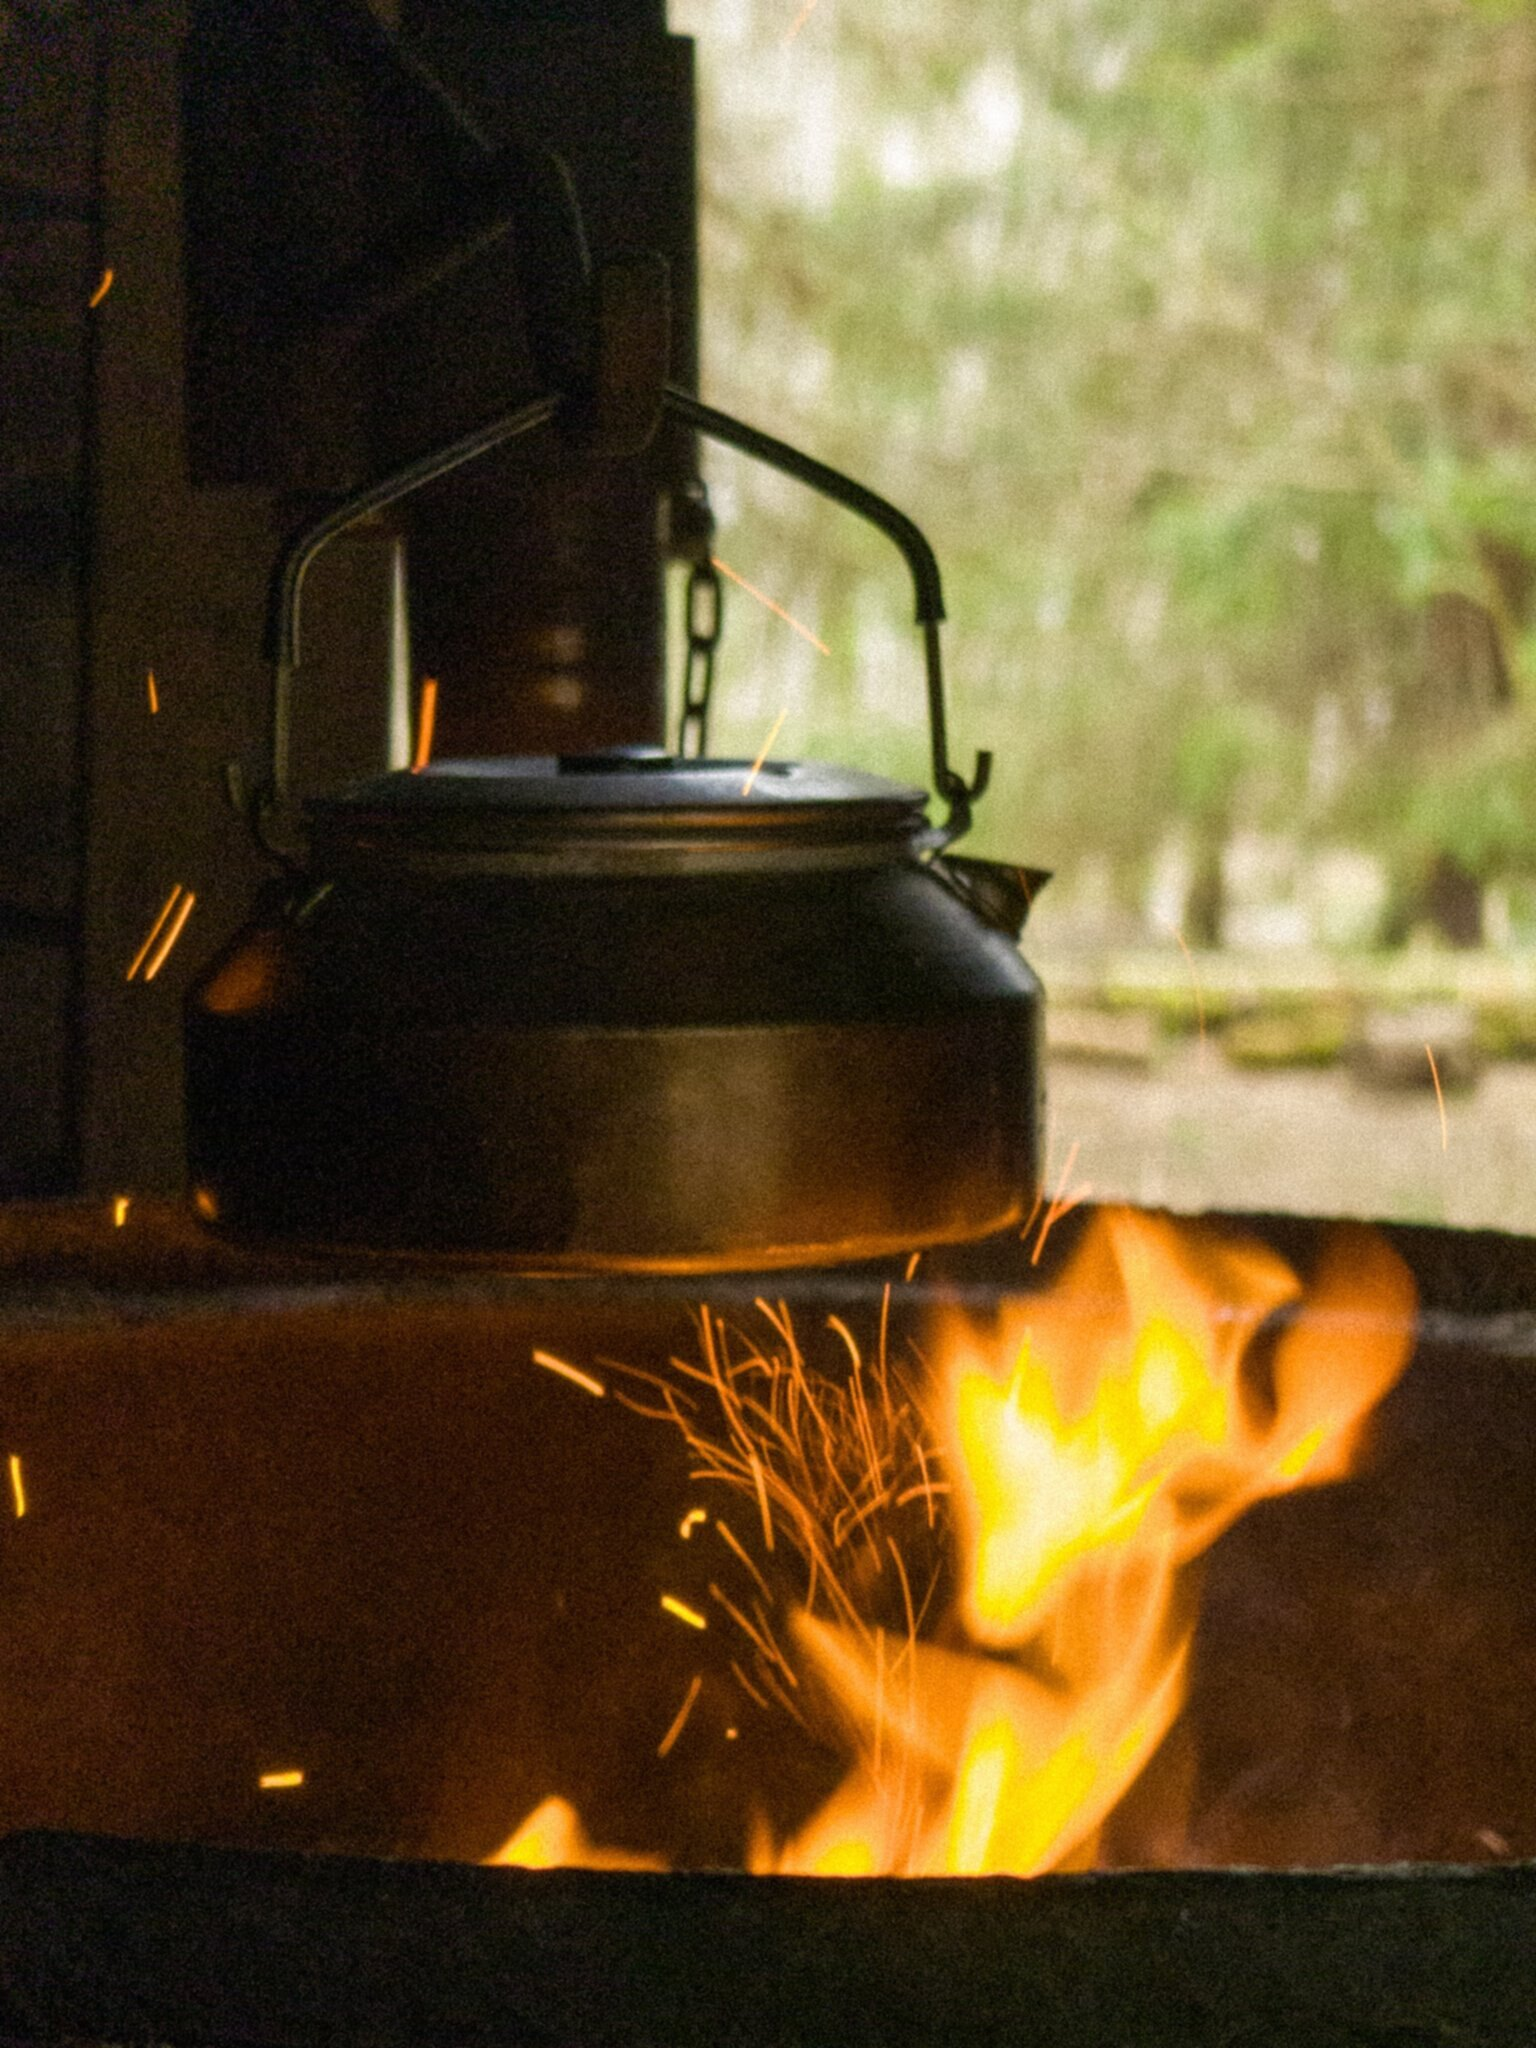
\includegraphics[height=0.9\linewidth]{assets/kuvakilpailu3}\\
	``Kahvii'' - Mikko% Niinimäki
\end{center}

\columnbreak

% \vspace*{-0.16cm}
	\subsection*{2. paikka:}
	\vspace*{0.54cm}
\begin{center}
	\noindent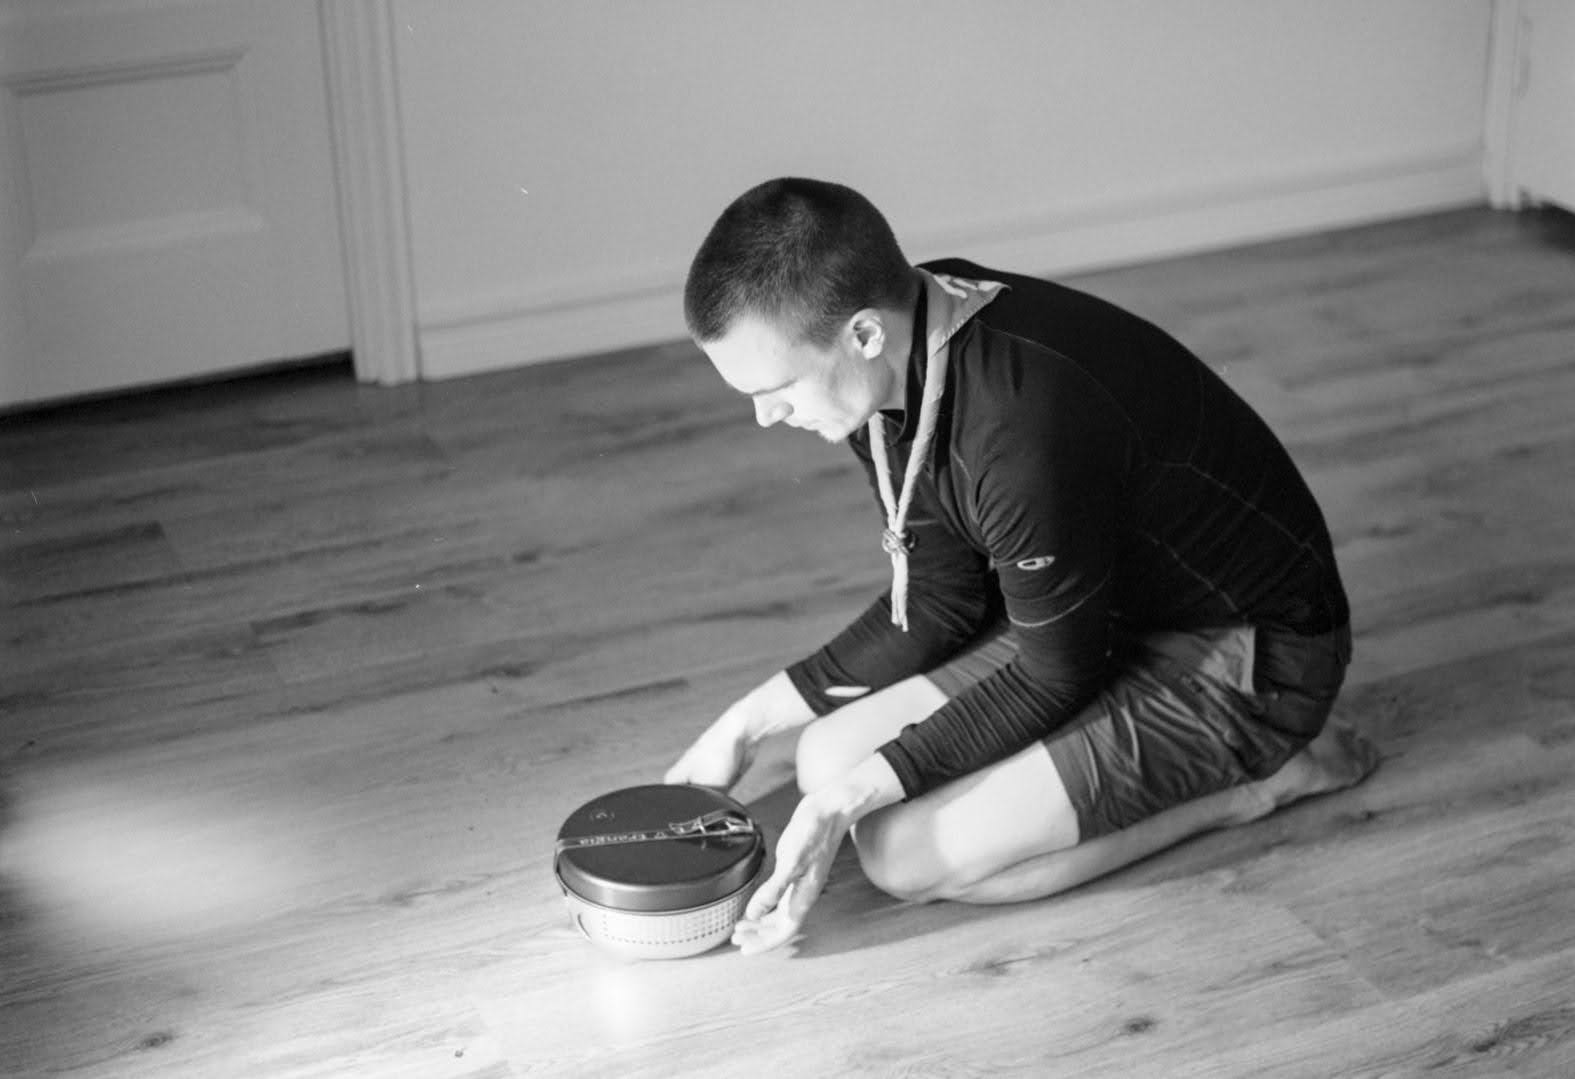
\includegraphics[width=0.99\linewidth]{assets/kuvakilpailu2}\\
	``Mies ja retkikeitin'' - Janne% Suomalainen
	\vspace*{0.54cm}
\end{center}

\end{multicols}

\begin{multicols}{2}

	\noindent Lähteet: \quad --

	\noindent Tuomariston keskiarvo: 2,5/5

	\columnbreak

	\noindent Lähteet: Poika ja pääkallo\\ \hfill - Magnus Enckell

	\noindent Tuomariston keskiarvo: 3,75/5

\end{multicols}

\begin{multicols}{2}

\noindent Kuva itsessään on oikein hieno ja se voisi sopia erinomaisesti Tassuun esim.
artikkelin kuvitukseksi. Kuva on sopivan yksinkertainen ja tunnelmallinen ja
kuvaa hyvin sitä, miltä kahvin juominen metsäretkellä tuntuu. Kuitenkin
kuvakilpailun tehtävänannon se ohittaa, sillä se ei viittaa mihinkään
taideteokseen, eikä näin ollen ole kilpailun sääntöjen mukainen.

	\columnbreak

\noindent Kuvan idea on luova ja kuvaan otettu retkikeitin myös lisää siihen
asiaankuuluvaa partiotunnelmaa. Asetelma mukailee hienosti alkuperäistä
taideteosta. Kuvan valotus on paikoittain hieman liian kirkas. Kuva on hyvin
yksinkertainen ja vaikka se ei olekaan huono asia, raati jäi kaipaamaan jotakin
elementtiä, joka olisi kiinnittänyt katsojan mielenkiinnon paremmin, minkä
vuoksi se jäi hitusen alle voittopisteiden.

\end{multicols}

\clearpage
% \vspace*{0.64cm}
\subsection*{1. paikka:}
\begin{center}
	\noindent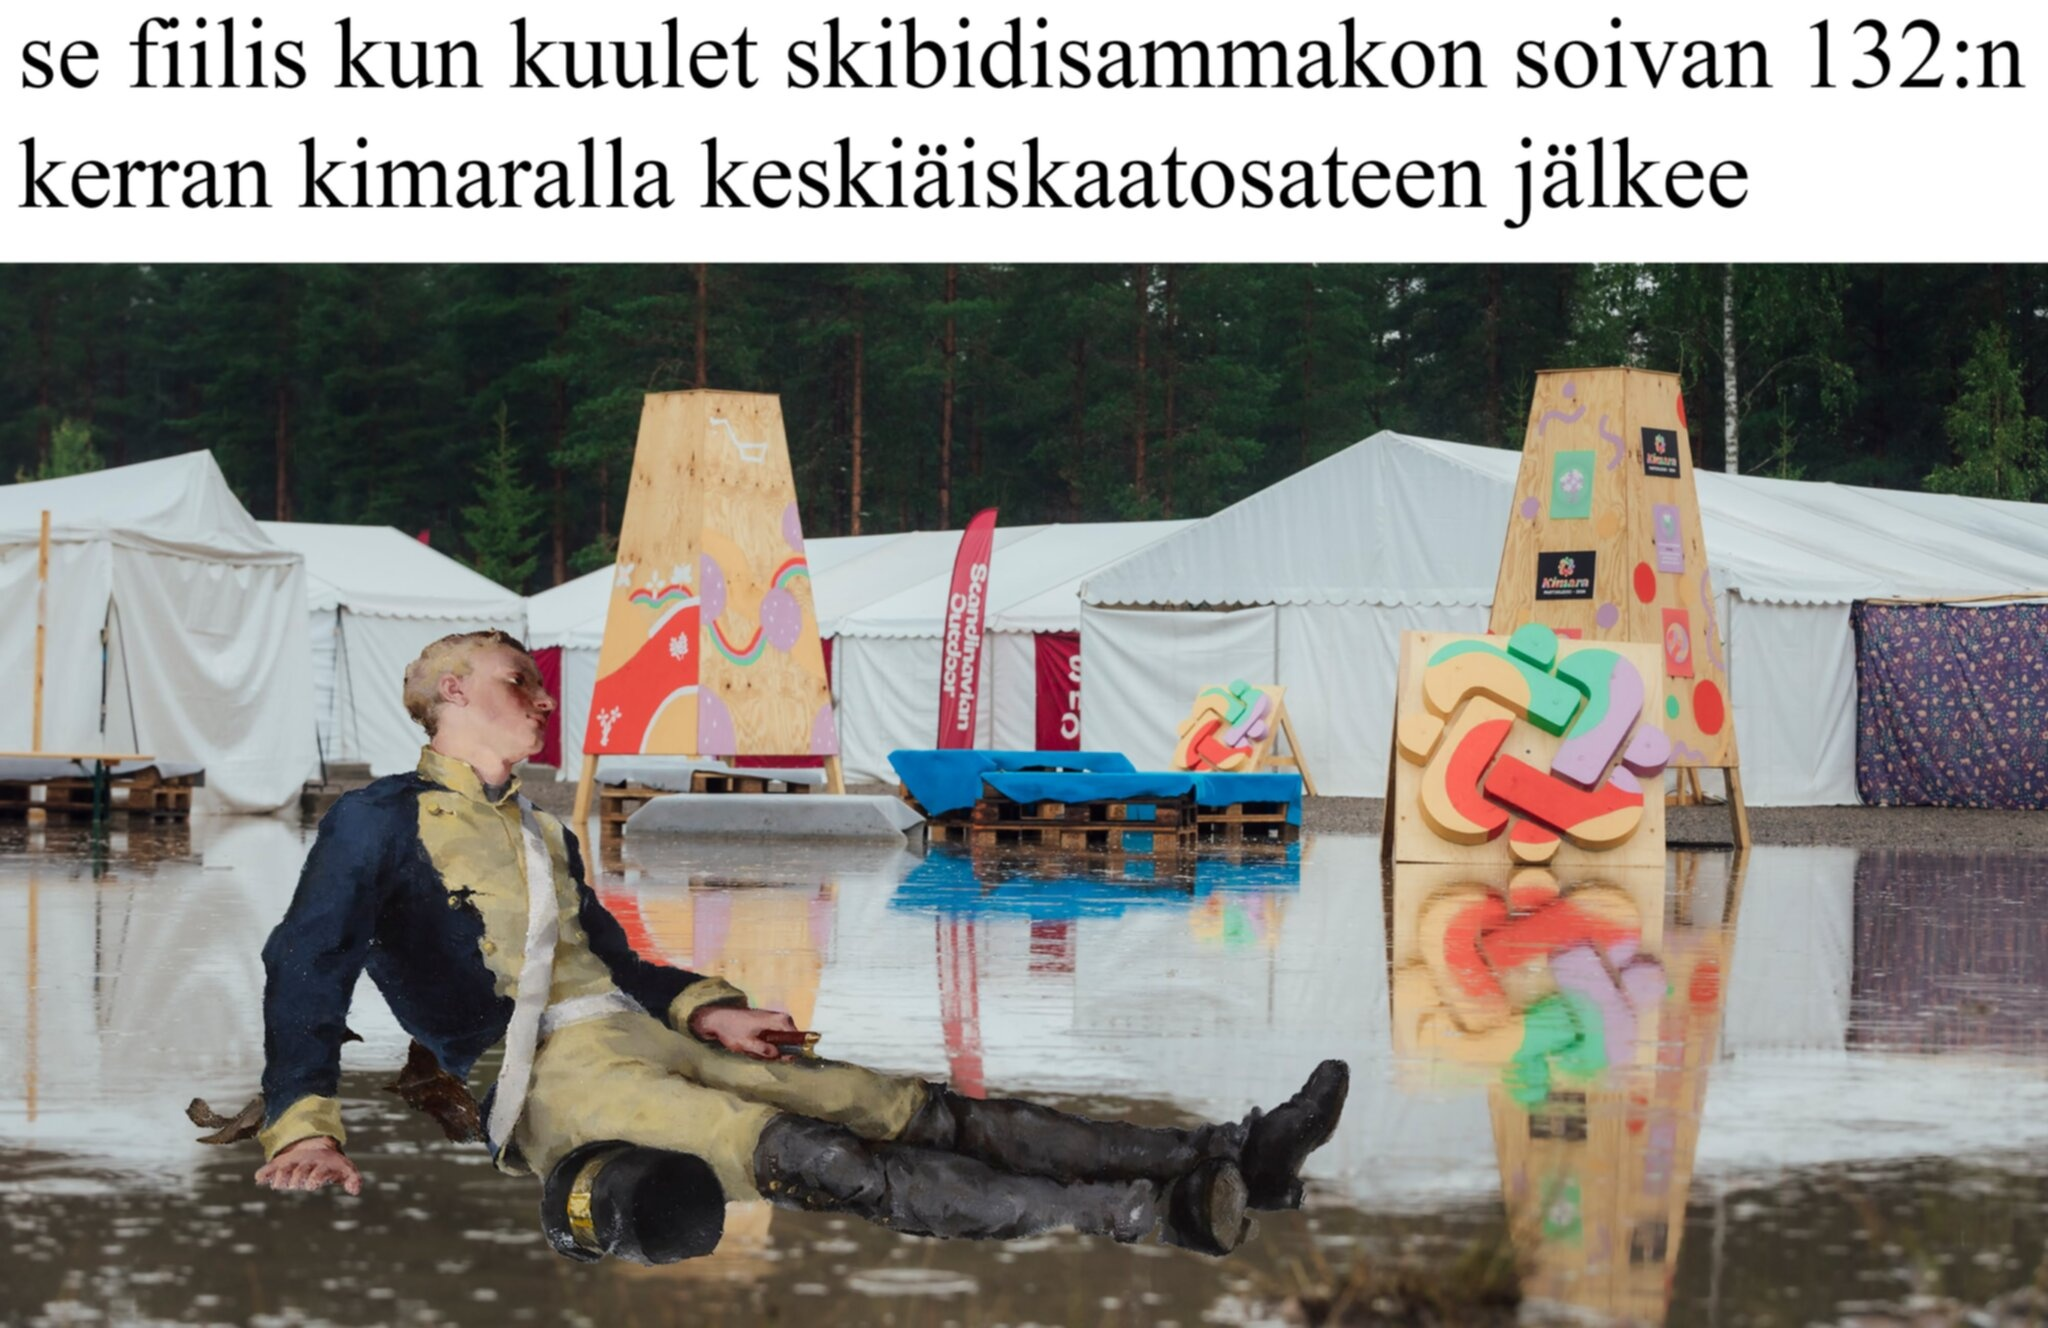
\includegraphics[width=1.0\linewidth]{assets/kuvakilpailu1}\\
	``rip bro.png'' - Alden% Forsström
\end{center}

\noindent Lähteet: \quad Haavoittunut Soturi Hangessa - Helene Schjerfbeck

\qquad\qquad Hanna Hämäläisen kuva, PäPa:n kuvapankistä

\bigskip
\noindent Tuomariston keskiarvo: 3,875/5\\
\noindent Eliaksen arvio: ``5/5 absolute cinema''

\bigskip
\noindent Kuva vetosi raatiin, sillä suurin osa pystyi samaistumaan siinä
kuvattuun tuskaan ja epätoivoon. Myös raadin iän ja kypsyyden huomioon ottaen
ei tule yllätyksenä, että meemiformaatti keräsi eniten pisteitä. Hauskuutta
kuvaan lisää se, että sen taustana on käytetty oikeaa kuvaa kuvatusta
tilanteesta. Tekijältä kuitenkin meni ohi oiva mahdollisuus käyttää numeroa
104, jolloin kuvasta olisi tullut entistä moniulotteisempi. Myös kuvatekstin
kielelliseen asuun olisi voinut panostaa enemmän. Kuva ei myöskään aukea
yleisölle, joka ei ollut Kimaralla kokemassa kuvattua tilannetta ja tästä
syystä myös tuomariston pisteiden keskiarvo laski.


% \clearpage\section{Tulossa pian}


\clearpage

\thispagestyle{empty}
% \ThisCenterWallPaper{1.07}{assets/no_auto_compression/takakansikuva.jpg}~

\vfill

\newtcolorbox{kuruboxendpage}[1][]{%
    enhanced,
    before skip=0mm,after skip=0mm, 
    width=0.68\textwidth, boxrule=0mm,
    colback=kuru, colframe=kuru, % Colors
    sharp corners,
    underlay={%
	    \fill[kuru] ([xshift=-8mm,yshift=3mm]frame.north west) -- ([yshift=1mm]frame.north east)
	    -- ([xshift=1mm,yshift=-3mm]frame.south east) -- ([xshift=-7mm,yshift=-1mm]frame.south west)
	    -- cycle;
	    \fill[white] ([xshift=-4mm,yshift=-1mm]frame.north west) ellipse (1mm and 2mm);
	    \fill[white] ([xshift=-1mm,yshift=-1mm]frame.north west) ellipse (1mm and 2mm);
	    \fill[white] ([xshift=-2.5mm,yshift=-5mm]frame.north west) circle (1mm);
	    \fill[white] ([xshift=-2.5mm,yshift=-8mm]frame.north west) circle (1mm);
        },
    % drop fuzzy shadow, % Shadow
    title={#1},
}

{
	\noindent
	\begin{addmargin}[0.32cm]{0cm}
		\begin{center}
			\begin{kuruboxendpage}[]
				\color{white}{\Large\bfseries 1/2025 Kurkisuon Rusakot ry}
			\end{kuruboxendpage}
		\end{center}
	\end{addmargin}
}
\end{document}
